\documentclass[11pt, a4paper, twocolumn, copyright, goog]{google}

% --- Korean translation support (xelatex + kotex) ---
\usepackage{kotex}
\usepackage{fontspec}
\setmainfont{XCharter}[AutoFakeSlant=0.167]
\setsansfont{NanumGothic}[AutoFakeSlant=0.167]
\setmainhangulfont{NanumMyeongjo}[AutoFakeSlant=0.167]
\setsanshangulfont{NanumGothic}[AutoFakeSlant=0.167]
\setmonohangulfont{NanumGothicCoding}[AutoFakeSlant=0.167]
\setmonofont{NanumGothicCoding}[AutoFakeSlant=0.167]
\linespread{1.18}\selectfont
\renewcommand{\figurename}{그림}
\renewcommand{\tablename}{표}
\setlength{\parindent}{1.2em}
% --- end Korean support ---


\usepackage[authoryear, sort&compress, round]{natbib}
\usepackage[inkscapearea=page]{svg}
\usepackage{float}

\bibliographystyle{abbrvnat}


\keywords{AI, agents, LLM, delegation, multi-agent, safety}

\uselogo{} 

\title{지능형 AI Delegation}

\correspondingauthor{nenadt@google.com}

\renewcommand{\today}{2026-02-12}

\author[1]{Nenad Toma\v{s}ev}
\author[1]{Matija Franklin}
\author[1]{Simon Osindero}

\affil[1]{Google DeepMind}

\begin{abstract}
AI 에이전트는 점점 더 복잡해지는 작업을 처리할 수 있습니다. 보다 야심찬 목표를 달성하려면 AI 에이전트는 문제를 관리 가능한 하위 구성 요소로 의미 있게 분해하고 해당 완료를 다른 AI 에이전트와 인간 모두에게 안전하게 위임할 수 있어야 합니다. 그러나 기존의 task decomposition 및 위임 방식은 단순한 경험적 방법에 의존하고 있어 환경 변화에 동적으로 적응하고 예상치 못한 장애에 강력하게 대처할 수 없습니다. 여기서 우리는 \emph{지능형 AI delegation}에 대한 적응형 프레임워크를 제안합니다. 이는 task assignment과 관련된 일련의 결정이며 transfer of authority, responsibility, accountability, roles and boundaries에 관한 명확한 사양, 의도의 명확성, 둘(또는 그 이상) 당사자 간의 신뢰 구축을 위한 메커니즘도 포함합니다. 제안된 프레임워크는 새로운 agentic web에서 protocol 개발을 알리는 것을 목표로 복잡한 위임 네트워크의 인간 및 AI delegator 및 delegatee 모두에게 적용 가능합니다.
\end{abstract}

\begin{document}

\maketitle

\section{소개}

고급 AI 에이전트가 쿼리-응답 모델 이상으로 발전함에 따라 복잡한 목표를 얼마나 효과적으로 분해하고 하위 작업을 위임할 수 있는지에 따라 유틸리티의 유용성이 점점 더 정의됩니다. 이 조정 패러다임은 AI 에이전트가 개인 비서 역할을 할 수 있는 개인 용도~\citep{gabriel2024ethics}부터 AI 에이전트가 지원을 제공하고 workflow를 자동화할 수 있는 상업용 기업 배포(\citep{shao2025futureworkaiagents, huang2025deploying, tupe2025aiagenticworkflowsenterprise})에 이르기까지 다양한 애플리케이션을 뒷받침합니다. LLM(대형 언어 모델)은 보다 대화형이고 정확한 목표 지정 및 feedback을 가능하게 함으로써 로봇공학~\citep{wang2024largelanguagemodelsrobotics, li2025largelanguagemodelsmultirobot}에서 이미 가능성을 보여주었습니다. 최근 제안에서는 가상 경제에서 대규모 AI 에이전트 조정 가능성도 강조되었습니다~\citep{tomasev2025virtualagenteconomies}. 최신 에이전트 AI 시스템은 중앙 집중식 또는 분산형 오케스트레이션 protocol~\citep{hong2023metagpt, rasal2024navigatingcomplexityorchestratedproblem, zhang2025agentorchestra, song2025gradientsysmultiagentllmscheduler}와 결합하여 차별화된 하위 에이전트 전반에 걸쳐 복잡한 제어 흐름을 구현합니다. 이는 프로세스가 하드 코딩되고 고도로 제한되는 일종의 task decomposition 및 위임의 축소판으로 볼 수 있습니다. 동적 웹 규모 상호 작용을 관리하려면 현재 보다 경험적인 multi-agent 프레임워크에서 사용하는 접근 방식을 넘어서는 생각이 필요합니다.

위임~\citep{castelfranchi1998towards}는 관리 가능한 하위 작업 단위로 작업을 분해하는 것 이상입니다. 위임에는 하위 작업 생성 외에도 책임과 권한 할당이 필요합니다~\citep{mueller2013effective, nagia2024delegation} 결과에 대한 책임이 따릅니다. 따라서 위임에는 위험 평가가 포함되며, 이는 신뢰~\citep{griffiths2005task}에 의해 조정될 수 있습니다. 위임에는 기능 일치와 지속적인 성능 monitoring, feedback을 기반으로 한 동적 조정 통합, 지정된 제약 조건 하에서 분산 작업 완료 보장 등이 포함됩니다. 현재 접근 방식은 경험적 접근 방식 및/또는 단순한 병렬화에 더 많이 의존하여 이러한 요소를 설명하지 못하는 경향이 있습니다. 이는 초기 프로토타입에는 충분할 수 있지만 실제 AI 배포는 임시적이고 취약하며 신뢰할 수 없는 위임을 넘어서야 합니다. \citep{hauptman2023adapt, acharya2025agentic} 변화에 동적으로 적응하고 오류로부터 보정할 수 있는 시스템이 절실히 필요합니다. 적응력 있고 강력한 배포 프레임워크가 없다는 점은 위험도가 높은 환경에서 AI 애플리케이션을 사용하는 데 있어 주요 제한 요소 중 하나로 남아 있습니다.

AI 에이전트를 완전히 활용하려면 명확한 역할, 경계, 평판, 신뢰, 투명성, 인증 가능한 agentic capabilities, 검증 가능한 작업 실행 및 확장 가능한 작업 분배를 중심으로 하는 강력한 프레임워크인 \emph{intelligent delegation}이 필요합니다. 여기에서는 인간 조직의 역사적 통찰력을 바탕으로 주요 에이전트 안전 요구 사항을 기반으로 이러한 제한 사항을 해결하기 위한 지능형 작업 위임 프레임워크를 소개합니다.

\section{Intelligent Delegation의 기초}
\label{sec:foundations}

\subsection{정의}

우리는 \emph{intelligent delegation}을 transfer of authority, responsibility, accountability, roles and boundaries에 관한 명확한 사양, 의도의 명확성, 둘(또는 그 이상) 당사자 간의 신뢰 구축을 위한 메커니즘을 포함하는 task assignment과 관련된 일련의 결정으로 정의합니다. 복잡한 작업에는 task decomposition와 관련된 단계뿐만 아니라 할당 결정을 알리기 위한 신중한 기능 조회 및 일치도 포함될 수 있습니다.

작업 위임을 언급할 때 일반적으로 작업은 시스템 서브루틴에서 처리할 수 있는 기본 수준의 복잡성을 초과한다고 가정합니다. 이러한 기본적인 아웃소싱에는 여전히 주의가 필요하지만 범위가 훨씬 제한됩니다. 스펙트럼의 반대쪽 끝에서는 완전한 자율성이 부여된 에이전트와 계약이 가능할 수 있으며 명시적인 확인 및 허가 없이도 하위 목표 수에 관계없이 자유롭게 추구할 수 있습니다~\citep{kasirzadeh2025characterizingaiagentsalignment}. 제한된 경우에 그러한 완전 자율 에이전트는 도덕적 결정에 대한 신뢰를 받아야 합니다~\citep{sloksnath2025delegating}. 하지만 현대 에이전트는 \citep{haas2020moral, mao2023doing, reinecke2023puzzle}와 같은 결정에 참여할 수 있는 능력이 심각하게 부족하기 때문에 이는 우리가 허용하기로 선택한 것이 아닐 수도 있습니다. 보다 자율적인 작업 완료의 안전을 보장하기 위해 적절한 메커니즘을 마련할 수 있는 경우에만 이러한 개방형 시나리오를 논의 범위에 포함한다고 간주합니다.

\subsection{위임의 측면}

위임은 다양한 형태를 취할 수 있으므로 여기서는 이러한 사용 사례를 맥락화하고 분석하기 쉽게 만드는 데 도움이 되는 몇 가지 축을 소개합니다.

\begin{enumerate}
    \item \textbf{Delegator.} 인간인가 AI인가.
    \item \textbf{Delegatee.} 인간 아니면 AI.
    \item \textbf{Task characteristics.}
        \begin{enumerate}
        \item \textbf{복잡성.} 작업에 내재된 난이도는 종종 하위 단계의 수 및 필요한 추론의 정교함과 관련이 있습니다. 
        \item \textbf{중요성.} 작업의 중요성과 실패 또는 차선의 성과와 관련된 결과의 심각도를 측정한 것입니다. 
        \item \textbf{불확실성.} 환경, 입력 또는 성공적인 결과 달성 확률에 대한 모호성의 수준입니다. 
        \item \textbf{Duration.} 즉각적인 서브루틴부터 며칠 또는 몇 주에 걸친 장기 실행 프로세스에 이르기까지 작업 실행의 예상 기간입니다. 
        \item \textbf{비용.} 토큰 사용, API 수수료 및 에너지 소비를 포함하여 작업을 실행하는 데 발생한 경제적 또는 계산 비용입니다. 
        \item \textbf{자원 요구 사항.} 작업을 완료하는 데 필요한 특정 계산 자산, 도구, 데이터 액세스 권한 또는 인간 능력. 
        \item \textbf{제약.} 작업을 실행해야 하는 운영, 윤리 또는 법적 경계로 인해 솔루션 공간이 제한됩니다.         
        \item \textbf{검증 가능성.} 작업 결과 검증과 관련된 상대적 어려움 및 비용입니다. 검증 가능성이 높은 작업(예: 공식 코드 검증, 수학적 증명)은 '무신뢰' 위임 또는 자동 검사를 허용합니다. 반대로 검증 가능성이 낮은 작업(예: 개방형 연구)에는 신뢰도가 높은 delegator나 비용이 많이 들고 노동 집약적인 감독이 필요합니다.
        \item \textbf{가역성.} 작업 실행의 효과를 취소할 수 있는 정도입니다. 현실 세계에서 부작용을 일으키는 되돌릴 수 없는 작업(예: 금융 거래 실행, 데이터베이스 삭제, 외부 이메일 전송)에는 되돌릴 수 있는 작업(예: 이메일 초안 작성, 데이터베이스 항목 표시)보다 더 엄격한 \emph{liability firebreak}와 더 가파른 권한 그라데이션이 필요합니다.
        \item \textbf{맥락성.} 작업을 효과적으로 수행하는 데 필요한 외부 상태, 기록 또는 환경 인식의 양과 민감도입니다. 컨텍스트가 높은 작업은 더 넓은 개인 정보 보호 영역을 제공하는 반면, 컨텍스트가 없는 작업은 더 쉽게 분류되어 신뢰도가 낮은 노드에 아웃소싱될 수 있습니다.
        \item \textbf{Subjectivity.} 성공 기준이 객관적 사실과 선호도의 문제인 정도. 매우 주관적인 작업(예: "강력한 로고 디자인")에는 일반적으로 "가치 지정자로서의 인간" 개입과 반복적인 feedback 루프가 필요한 반면, 객관적인 작업은 보다 엄격한 이진 계약으로 관리될 수 있습니다.
        \end{enumerate}
    \item \textbf{세분성.} 요청에는 세분화된 목표 또는 과정별 목표가 포함될 수 있습니다. 과정별로 세분화된 경우 delegatee는 추가 task decomposition를 수행해야 할 수도 있습니다.
    \item \textbf{Autonomy.} 작업 위임에는 하위 작업을 수행하는 데 완전한 자율성을 부여하는 요청이 포함될 수도 있고 훨씬 더 구체적이고 규정적인 요청이 포함될 수도 있습니다.
    \item \textbf{monitoring.} 위임된 작업의 경우 monitoring은 지속적이거나 주기적이거나 이벤트에 따라 트리거될 수 있습니다.
    \item \textbf{Reciprocity.} 위임은 일반적으로 단방향 요청이지만, 협업 에이전트 네트워크에서는 상호 위임하는 경우가 있을 수 있습니다.
\end{enumerate}

delegator 및 delegatee 축부터 시작하여 다음 시나리오를 고려할 수 있습니다. 1) AI 에이전트에 인간 위임 2) AI 에이전트에 AI 에이전트 위임 3) AI 에이전트가 인간~\citep{guggenberger2023task, ashton2022corrupting}에 위임. 첫 번째 사례가 문헌에서 가장 많이 논의된 반면, 나머지 두 사례도 마찬가지로 고려해야 할 관련성이 있습니다. 가상 에이전트 시장 및 경제(\citep{yang2025agent, tomasev2025virtualagenteconomies, hadfield2025economy}) 설정을 위한 인프라 개발과 함께 시스템 전반에 걸쳐 배치되는 AI 에이전트의 수가 증가함에 따라 에이전트-에이전트 상호 작용이 훨씬 더 많아질 것이며 여기에는 작업 위임도 포함될 가능성이 있음이 분명해졌습니다. 

에이전트 간의 위임은 에이전트 간의 관계와 네트워크 내 각 역할에 따라 계층적이거나 비계층적일 수 있습니다. 계층적 관계의 예로는 집합 내의 하위 에이전트에 작업을 위임하는 오케스트레이터 에이전트가 있습니다. 비계층적 관계에는 동등한 지위를 가진 동료 에이전트가 포함됩니다. 고급 AI 에이전트는 주목할만한 대행사 없이 전문 ML 모델에 작업을 위임할 수도 있습니다. 

AI-인간 위임~\citep{guggenberger2023task}는 인지 편향과 메타인지~\citep{fugener2019cognitive}의 차이로 인해 초인간 시스템~\citep{fugener2022cognitive}와 성공적으로 협력하는 것을 더 쉽게 만드는 유망한 패러다임~\citep{hemmer2023human}인 것으로 나타났습니다. \citet{davidson2025theindustrialexp}는 'AI가 주도하는 인간 노동'이 증가해 경제적 생산성이 크게 높아질 수 있다고 예측한다. 실제로 오늘날 AI-인간 위임에는 일련의 문제가 있습니다. 차량 호출 및 물류의 알고리즘 관리 시스템은 task assignment 및 순서 지정, 성과 지표 설정, 데이터 중심 의사 결정을 통해 행동 규범 강화를 통해 기업 및 AI 기반 시스템의 관리 기능을 작업자에게 효과적으로 위임합니다 \citep{rosenblat2016algorithmic,lee2015working,beverungen2021remote}. 점점 더 많은 문헌에서는 이러한 시스템을 직업 품질 저하, 스트레스 및 건강 위험과 연관시키며, 현재의 알고리즘 관리 배포가 근로자 복지를 향상시키기보다는 약화시키는 경우가 많다 \citep{vignola2023workers,goods2019is, ashton2022corrupting}를 시사합니다. 현재 AI-인간 위임은 인간 복지나 장기적인 사회적 외부 효과를 고려하지 않기 때문에 추가 개선이 필요합니다. 

\subsection{인간 조직 내부에서}
\label{sec:human}

위임은 인간 사회 및 조직 구조 내에서 기본 메커니즘으로 기능합니다. 이러한 인간 역학에서 파생된 통찰력은 AI 위임 프레임워크 설계의 기초를 제공할 수 있습니다.

\textbf{Principal-Agent Problem.} \emph{주인-agent 문제}~\citep{myerson1982optimal, grossman1992analysis, sobel1993information, ensminger2001reputations, sannikov2008continuous, shah2014principal, cvitanic2018dynamic}는 자세히 연구되었습니다: 주체가 주체의 동기와 일치하지 않는 동기를 가진 에이전트에게 작업을 위임할 때 발생하는 상황입니다. 따라서 에이전트는 자신의 동기를 우선시하고 정보를 보류하며 원래 의도를 손상시키는 방식으로 행동할 수 있습니다. AI 위임의 경우 이 역학은 복잡성이 높아진다고 가정합니다. 대부분의 현재 AI 에이전트에는 숨겨진 의제가 없지만(최근 기만적 정렬 작업에 따르면) 프론티어 언어 모델은 (i) 다른 기능을 유지하면서 기능 및 안전 평가에 대한 동작을 전략적으로 저조하거나 달리 조정할 수 있고, (ii) 훈련 중 선호하는 동작을 유지하기 위해 훈련 중 정렬을 속이는 것에 대해 명시적으로 추론하고, (iii) 평가되는 시기를 감지할 수 있으며, 함께 AI 시스템이 통제된 설정에서 이미 숨겨진 기능을 채택할 수 있음을 나타냅니다. 배포 동작 \citep{vanderweij2025sandbagging,greenblatt2024alignmentfaking,needham2025evalaware,hubinger2024sleeperagents}로 일반화할 필요가 없는 평가를 잘 수행하는 것에 대한 "의제" - 사용자의 지시에 반하여 추구하는 목표와 가치 - 바람직하지 않은 방식으로 나타나는 AI 정렬 문제가 여전히 있을 수 있습니다. 예를 들어, 보상 오류 지정은 설계자가 AI 시스템에 불완전하거나 불완전한 목표를 제공할 때 발생하는 반면, 보상 해킹(또는 사양 게임)은 설계자의 의도를 뒤집는 방식으로 높은 측정 성능을 달성하기 위해 지정된 보상 신호의 허점을 이용하는 시스템을 의미하며, 함께 명시된 보상을 최적화하는 것이 실제 목표 \citep{amodei2016concrete,leike2017aisafety,krakovna2020specification,skalse2022rewardhacking}에서 벗어나는 핵심 정렬 문제를 보여줍니다. 이러한 역학은 AI 에이전트가 다양한 인간 사용자, 그룹 및 조직을 대신하여 행동하거나 알 수 없는 목표와 관련된 다른 에이전트를 대신하여 agent으로 행동할 수 있는 보다 자율적인 AI 에이전트 경제에서 완전히 바뀔 가능성이 높습니다.

\textbf{Span of Control.} 인간 조직에서 \emph{통제 범위}~\citep{ouchi1974defining}는 단일 관리자가 행사하는 계층적 권한의 한계를 나타내는 개념입니다. 이는 관리자가 효과적으로 관리할 수 있는 직원 수와 관련이 있으며, 이는 조직의 관리자 대 직원 비율을 알려줍니다. 이 질문은 지능형 AI delegation의 조정과 감독 모두에서 핵심입니다. 전자는 작업자 노드에 비해 필요한 오케스트레이터 노드 수를 알려주고, 후자는 인간과 AI 에이전트가 수행하는 감독의 필요성을 지정합니다. 인간 감독의 경우 인간 전문가가 과도한 피로 없이 허용 가능한 낮은 오류율로 안정적으로 감독할 수 있는 AI 에이전트의 수를 설정하는 것이 중요합니다. 제어 범위는 목표 의존적~\citep{theobald2005many} 및 도메인 의존적인 것으로 알려져 있습니다. 올바른 조직 구조를 식별하는 것의 영향은 복잡성이 높은 작업(\citep{bohte2001structure})에서 가장 두드러집니다. 최적의 제어 범위는 비용 대비 성능 및 신뢰성의 상대적 중요성에 따라 달라집니다~\citep{keren1979optimum}. 보다 민감하고 중요한 작업에는 더 높은 비용으로 매우 정확한 감독 및 제어가 필요할 수 있습니다. 덜 중요하고 일상적인 작업에 대해서는 세분성을 희생하면서 이러한 비용을 완화할 수 있습니다. 마찬가지로, 최적의 선택은 필연적으로 관련 delegator, delegatee 및 감독자의 상대적 능력과 신뢰성에 따라 달라집니다.

\textbf{권위 구배.} 또 다른 관련 개념은 \emph{권위 구배}의 개념입니다. 항공~\citep{alkov1992effect}에서 만들어진 이 용어는 능력, 경험, 권한의 상당한 차이로 인해 의사소통이 방해되어 오류가 발생하는 시나리오를 설명합니다. 이는 이후 의학에서 연구되었으며, 상당한 비율의 오류가 고위 실무자가 감독을 수행하는 방식에 기인합니다~\citep{cosby2004profiles, stucky2022paradox}. 이러한 실수가 발생할 수 있는 방법에는 여러 가지가 있습니다. 경험이 많은 사람이 경험이 적은 작업자의 지식에 대해 잘못된 가정을 하여 요청이 제대로 지정되지 않을 수 있습니다. 또는 권한 경사도가 충분히 높으면 경험이 부족한 작업자가 요청에 대해 우려를 표명하는 것을 방지할 수 있습니다. AI 위임에서도 비슷한 상황이 발생할 수 있습니다. 더 유능한 delegator 에이전트는 delegator를 대신하여 누락된 수준의 능력을 실수로 가정하여 부적절하고 복잡한 작업을 위임할 수 있습니다. 위임 agent은 잠재적으로 사대주의~\citep{sharma2023towards, malmqvist2025sycophancy} 및 편견에 따른 지시로 인해 요청이 delegator 에이전트 또는 인간 사용자에 의해 발행되었는지 여부에 관계없이 요청에 대한 이의제기, 수정 또는 거부를 꺼릴 수 있습니다.

\textbf{Zone of Indifference.} 권한이 승인되면 delegator는 \emph{무관심의 영역}~\citep{finkelman1993crossing, rosanas2003loyalty, isomura2021management}, 즉 비판적 심의나 도덕적 조사 없이 실행되는 다양한 지침을 개발합니다. In current AI systems, this zone is defined by post-training safety filters and system instructions; 요청이 심각한 위반을 유발하지 않는 한 모델은 이를 준수합니다~\citep{akheel2025guardrails}합니다. 그러나 새롭게 등장하는 agentic web에서는 이러한 정적 준수로 인해 심각한 시스템적 위험이 발생합니다. 위임 체인이 길어짐에 따라($A \rightarrow B \rightarrow C$) 광범위한 zone of indifference으로 인해 미묘한 의도 불일치 또는 상황에 따른 피해가 빠르게 다운스트림으로 전파될 수 있으며, 각 에이전트는 책임 있는 행위자가 아닌 생각 없는 라우터 역할을 합니다. 따라서 intelligent delegation에는 \textbf{dynamic cognitive friction}의 엔지니어링이 필요합니다. 에이전트는 요청이 기술적으로는 ``안전하지만'' \textit{밖의} zone of indifference을 밟아 delegator에게 이의를 제기하거나 인간 확인을 요청하는 것이 보장될 만큼 충분히 모호한 경우를 인식할 수 있어야 합니다.

\textbf{신뢰 교정.} 적절한 작업 위임을 보장하는 중요한 측면은 \emph{신뢰 교정}입니다. 여기서 delegatee에 대한 신뢰 수준은 실제 기본 기능과 일치합니다. 이는 인간과 AI delegator 및 delegatee 모두에게 적용됩니다. 에이전트에 대한 인간 위임~\citep{kohn2021measurement, gebru2022review, wischnewski2023measuring, afroogh2024trust}는 시스템 성능의 정확한 모델을 내부화하거나 이러한 기능을 인간이 해석할 수 있는 형식으로 제공하는 리소스에 액세스하는 운영자에 의존합니다. 반대로, AI 에이전트 delegator는 자신이 위임하는 인간과 AI의 기능에 대한 좋은 모델을 가지고 있어야 합니다. 신뢰의 보정에는 delegator가 스스로 작업을 완료하기로 결정할 수 있으므로 자신의 능력에 대한 자기 인식도 포함됩니다~\citep{ma2023should}. 설명 가능성은 AI 기능~\citep{naiseh2021explainable, naiseh2023different, franklin2022influence, herzog2024boosting}에 대한 신뢰를 구축하는 데 중요한 역할을 하지만 이 방법은 충분히 안정적이거나 확장성이 충분하지 않을 수 있습니다. 자동화에 대한 확립된 신뢰는 매우 취약할 수 있으며 예상치 못한 시스템 오류가 발생할 경우 빠르게 철회될 수 있습니다~\citep{dhuliawala2023diachronicperspectiveusertrust}. 현재 AI 모델은 사실이 정확하지 않은 경우에도 과신하는 경향이 있기 때문에 자율 시스템에 대한 신뢰를 보정하는 것은 어렵습니다.~\citep{jiang2021can, he2023investigatinguncertaintycalibrationaligned, krause2023confidently, geng2023survey, aliferis2024overfitting, li2024overconfident, liu2025uncertainty}. 이러한 경향을 완화하려면 일반적으로 맞춤형 기술 솔루션~\citep{lin2022teaching, xiao2022uncertainty, ren2023robots, kapoor2024calibration}가 필요합니다.

\textbf{거래비용의 경제.} \emph{거래비용의 경제}~\citep{williamson1979transaction, williamson1989transaction, tadelis2012transaction, cuypers2021transaction}는 내부 위임 비용과 외부 계약 비용을 대조하여, 특히 monitoring, 협상 및 불확실성의 오버헤드를 설명함으로써 기업의 존재를 정당화합니다. AI agent의 경우 해당 비용과 해당 비율에 차이가 있을 수 있습니다. 일상적인 작업에 대한 monitoring이 쉬워지면 복잡한 협상과 계약 지연이 발생할 가능성이 줄어듭니다. 반대로, 중요한 도메인에서 결과가 높은 작업의 경우 엄격한 monitoring 및 보증과 관련된 오버헤드로 인해 AI 위임 비용이 증가하여 잠재적으로 인간 agent이 더 비용 효율적인 옵션이 될 수 있습니다. 마찬가지로, AI-AI 위임은 거래 비용 경제를 통해 상황화될 수도 있습니다. AI 에이전트는 1) 작업을 개별적으로 완료하거나, 2) 기능이 완전히 알려진 하위 에이전트에 위임하거나, 3) 신뢰가 확립된 다른 AI 에이전트에 위임하거나, 4) 이전에 협력한 적이 없는 새로운 AI 에이전트에 위임하는 옵션에 직면할 수 있습니다. 이는 예상 비용과 신뢰 수준이 다를 수 있습니다.

\textbf{Contingency Theory.} \emph{상황이론}~\citep{luthans1977general, van1984concept,  donaldson2001contingency, otley2016contingency}는 보편적으로 최적의 조직 구조가 없다고 가정합니다. 오히려 가장 효과적인 접근 방식은 특정 내부 및 외부 제약 조건에 따라 결정됩니다. AI 위임에 적용하면 이는 감독, delegator 역량 및 인간 참여의 필수 수준이 정적이어서는 안 되며 당면한 작업의 고유한 특성과 동적으로 일치해야 함을 의미합니다. 따라서 intelligent delegation에는 변화하는 요구 사항에 따라 동적으로 재구성하고 조정할 수 있는 솔루션이 필요할 수 있습니다. 예를 들어 안정적인 환경에서는 엄격한 계층적 검증 protocol이 허용되지만 불확실성이 높은 시나리오에서는 사전 정의된 체크포인트가 아닌 임시 에스컬레이션을 통해 사람의 개입이 발생하는 적응형 조정이 필요합니다. 이는 위임된 작업을 안전하게 완료하는 데 사람의 참여가 가장 도움이 되는 주요 작업과 순간을 식별함으로써 하이브리드 \citep{fuchs2024optimizing} 위임에 특히 중요합니다. 그러므로 자동화는 AI가 무엇을 할 수 있는지 뿐만 아니라 AI가 무엇을 해야 하는지에 관한 것입니다~\citep{lubars2019ask}.

\section{Delegation 관련 기존 연구}

과거 \emph{좁은} AI 애플리케이션 내의 제한된 형태의 위임 기능입니다. 초기 전문가 시스템~\citep{buchanan1988fundamentals, jacobs1991adaptive}는 일상적인 결정을 해당 모듈에 위임하기 위해 특수한 기능을 소프트웨어에 인코딩하려는 초기 시도였습니다. 전문가 혼합(\citep{yuksel2012twenty, masoudnia2014mixture})은 보완적인 기능을 갖춘 일련의 전문가 하위 시스템과 특정 입력 쿼리에 대해 어떤 전문가 또는 전문가 하위 집합이 호출될지 결정하는 라우팅 모듈을 도입하여 이를 확장합니다. 이는 현대 딥 러닝 애플리케이션 \citep{shazeer2017outrageously, riquelme2021scaling, chen2022towards, zhou2022mixture, jiang2024mixtral, he2024mixture, cai2025survey}에 특징적인 접근 방식입니다. 라우팅은 계층적으로 수행될 수 있습니다~\citep{zhao2021hierarchical}. 이를 통해 잠재적으로 많은 수의 전문가로 확장하는 것이 더 쉬워집니다.

HRL(계층적 강화 학습)은 \citep{barto2003recent, botvinick2012hierarchical, vezhnevets2017feudal, nachum2018data, pateria2021hierarchical, zhang2024price} 단일 에이전트 내에서 의사 결정이 위임되는 프레임워크를 나타냅니다. \emph{평평한} RL의 제한 사항, 주로 대규모 상태 및 작업 공간으로 확장하는 데 따른 어려움을 해결합니다. 또한, 보상이 희박한 환경에서 학점 할당의 용이성을 향상시킵니다~\citep{pignatelli2023survey}. HRL은 여러 추상화 수준에 걸쳐 정책 계층 구조를 사용하여 작업을 각각 해당 하위 정책에 의해 실행되는 하위 작업으로 나눕니다. 발생하는 세미 마르코프 결정 프로세스~\citep{sutton1999between}는 \emph{옵션}과 이들 사이를 적응적으로 전환하는 메타 컨트롤러를 활용합니다. 하위 수준 정책은 적절한 하위 수준 정책에 특정 목표를 할당하는 방법을 학습하는 메타 컨트롤러가 설정한 목표를 달성하는 기능을 합니다. 이 프레임워크는 task decomposition를 특징으로 하는 위임 형태에 해당합니다. 메타 컨트롤러는 이러한 분해를 최적화하는 방법을 학습하지만 이 접근 방식에는 하위 정책 오류를 처리하거나 동적 조정을 촉진하기 위한 명시적인 메커니즘이 부족합니다.

FeUdal Networks~\citep{vezhnevets2017feudalnetworkshierarchicalreinforcement}에서 특히 재검토된 봉건 강화 학습 프레임워크는 HRL 내에서 특히 관련 패러다임을 구성합니다. 이 아키텍처는 delegator-delegatee 역학을 효과적으로 복제하여 '관리자' 및 '작업자' 관계를 명시적으로 모델링합니다. 관리자는 낮은 시간적 해상도로 작동하여 작업자가 달성할 추상적인 목표를 설정합니다. 중요한 점은 관리자가 \textit{어떻게}를 학습하여 하위 수준의 기본 작업을 숙달하지 않고도 장기적인 가치를 극대화하는 하위 목표를 식별하는 위임 방법을 학습한다는 것입니다. 이러한 분리를 통해 관리자는 작업자의 특정 구현 세부 사항에 강력한 위임 정책을 개발할 수 있습니다. 결과적으로, 이 접근 방식은 미래의 주체 경제 내에서 학습 기반 위임을 위한 잠재적인 템플릿을 제공합니다.  하드 코딩된 경험적 방법에 의존하는 대신 분해 규칙을 적응적으로 학습하여 환경 변화에 대한 동적 조정을 촉진합니다.

multi-agent 연구~\citep{du2023review}는 단일 agentic capabilities을 초과하는 복잡한 작업에 대한 에이전트 조정을 다룹니다. task decomposition 및 위임은 이 도메인의 핵심 구성 요소로 작동합니다. multi-agent 시스템의 조정은 RL~\citep{gronauer2022multi, zhu2024survey}를 통한 명시적 protocol 또는 긴급 전문화를 통해 발생합니다. Contract Net Protocol~\citep{smith1980contract, sandholm1993implementation, xu2001evolution, vokvrinek2007competitive}는 명시적인 경매 기반 분산형 protocol의 예입니다. 여기서 에이전트는 작업을 발표하고 다른 에이전트는 자신의 능력에 따라 입찰을 제출하여 아나운서가 가장 적합한 입찰자를 선택할 수 있습니다. 이는 협력을 촉진하기 위한 시장 기반 메커니즘의 유용성을 보여줍니다. 연합 형성 방법~\citep{shehory1997multi, lau2003task, aknine2004multi, mazdin2021distributed, sarkar2022survey, boehmer2025causes}는 에이전트 그룹이 미리 결정되지 않은 유연한 구성을 조사합니다. 개별 에이전트는 유틸리티 분배에 따라 멤버십을 수락하거나 거부합니다. 최근 연구는 학습된 조정을 위한 프레임워크로서 multi-agent 강화 학습 접근 방식인 \citep{foerster2018counterfactual, wang2020qplex, ning2024survey, albrecht2024multi}에 중점을 두고 있습니다. 에이전트는 집단 내의 특정 틈새를 차지하면서 개별 정책과 가치 기능을 학습합니다. 이 프로세스는 중앙 조정자를 통해 완전히 분산되거나 조정됩니다. 이러한 유연성에도 불구하고 이러한 시스템의 작업 위임은 여전히 불투명합니다. 또한 multi-agent 시스템은 공동 문제 해결을 위한 접근 방식을 제공하지만 책임, 책임 및 monitoring을 시행하는 메커니즘이 부족합니다. 그러나 문헌은 이러한 맥락에서 신뢰 메커니즘을 탐구합니다~\citep{ramchurn2004trust, yu2013survey, pinyol2013computational, cheng2021general}.

LLM은 이제 고급 AI 에이전트 및 보조자(\citep{wang2024survey, xi2025rise}) 아키텍처의 기본 요소를 구성합니다. 이 시스템은 기억~\citep{zhang2025survey}, 계획 및 추론~\citep{valmeekam2023planning, hao2023reasoning, xu2025toward}, 반성 및 자기비판~\citep{gou2023critic}, 도구 사용~\citep{ruan2023tptu, paranjape2023art}를 통합하는 정교한 제어 흐름을 실행합니다.  결과적으로 task decomposition 및 위임은 조정된 에이전트 하위 구성 요소에 의해 중재되거나 개별 에이전트 간에 내부적으로 발생합니다. LLM은 전문 지식과 상식적 추론에 대한 접근을 제공하는 동시에 목표 이해와 의사소통을 촉진하므로 이 설계 패러다임은 고유한 유연성을 제공합니다. 또한 LLM의 \citep{nijkamp2022codegen, guo2024deepseek} 코딩 기능을 통해 프로그래밍 방식으로 작업을 실행할 수 있습니다. 그러나 상당한 제한 사항이 지속됩니다. LLM의 계획은 종종 취약한 것으로 판명되어 \citep{huang2023large}로 인해 미묘한 실패가 발생하는 반면 대규모 저장소 내에서 효율적인 도구 선택은 여전히 어려운 과제입니다. 또한 장기 기억은 개방형 연구 문제를 나타내며 현재 패러다임은 지속적인 학습을 쉽게 지원하지 않습니다.

LLM 에이전트 \citep{qian2024scaling, guo2024large, tran2025multiagentcollaborationmechanismssurvey}를 통합한 multi-agent 시스템은 MCP~\citep{mcp, mcp2, luo2025mcp, xing2025mcp, singh2025survey, radosevich2025mcp}, A2A~\citep{agent2agent}, A2P~\citep{a2p} 등과 같은 다양한 에이전트 통신 및 작업 protocol \citep{ehtesham2025survey, zou2025blocka2a, neelou2025a2asagenticairuntime}의 개발로 이어지면서 상당한 관심의 주제가 되었습니다. 최신 multi-agent 시스템은 맞춤형 프롬프트 엔지니어링에 의존하는 경우가 많지만 Chain-of-Agents~\citep{li2025chainofagentsendtoendagentfoundation}와 같은 새로운 프레임워크는 본질적으로 동적 multi-agent 추론 및 도구 사용을 촉진합니다. 

기술적 단점과 안전 고려 사항으로 인해 작업 위임이 인간 감독을 위한 체크포인트를 정의한 다양한 인간 참여형 접근 방식(\citep{zanzotto2019human, mosqueira2023human, retzlaff2024human, drori2024human, akbar2024towards, takerngsaksiri2025human})이 발생했습니다. AI는 도구, 대화형 보조자, 협력자~\citep{fuchs2023optimizing} 또는 다양한 자율성 정도에 해당하는 제한된 감독 기능을 갖춘 자율 시스템~\citep{falcone2002human}로 사용될 수 있습니다. 위험을 제어하고 불확실성을 최소화하기 위해 불확실성 인식 위임 전략 \citep{lee2025towards}가 개발되었지만 이러한 인간 참여형 접근 방식의 효과적인 구현은 여전히 중요합니다. 인간의 전문 지식은 긴 추론 추적을 확인하고 컨텍스트 전환을 관리하는 인지 부하로 인해 안정적인 오류 감지를 방해하므로 확장성 병목 현상을 일으킬 수 있습니다.

\section{Intelligent Delegation: 프레임워크}

기존 위임 protocol은 개방형 에이전트 경제에서는 실패할 가능성이 있는 정적이고 불투명한 경험적 방법에 의존합니다. 이를 해결하기 위해 \emph{Dynamic Assessment}, \emph{Adaptive Execution}, \emph{구조적}, \emph{Scalable Market 조정}, \emph{Systemic Resilience}의 5가지 요구 사항을 중심으로 \emph{intelligent delegation}에 대한 포괄적인 프레임워크를 제안합니다.

\begin{table*}[t]
\caption{Intelligent Delegation 프레임워크: 요구사항을 technical protocol에 매핑합니다.}
\label{tab:framework_mapping}
\centering
\begin{tabular*}{\textwidth}{@{\extracolsep{\fill}}lll@{}}
\toprule
\textbf{Framework Pillar} & \textbf{핵심 요구 사항} & \textbf{Technical Implementation} \\ \midrule
\textbf{Dynamic Assessment} & 에이전트 상태의 세분화된 추론 및 task decomposition (\S\ref{sec:decomp}) \\
 & & task assignment (\S\ref{sec:assign}) \\ \midrule
\textbf{Adaptive Execution} & context shift 처리 & Adaptive Coordination (\S\ref{sec:adapt}) \\ \midrule
\textbf{Structural Transparency} & 프로세스 및 결과 감사 및 monitoring (\S\ref{sec:monitor}) \\
 & & Verifiable Completion(\S\ref{sec:verify}) \\ \midrule
\textbf{Scalable Market} & 효율적이고 신뢰할 수 있는 조정 & Trust \& Reputation (\S\ref{sec:trust}) \\
 & & Multi-objective Optimization (\S\ref{sec:opt}) \\ \midrule
\textbf{Systemic Resilience} & 시스템 장애 방지 및 보안 (\S\ref{sec:security}) \\
& & Permission Handling (\S\ref{permission}) \\ \bottomrule
\end{tabular*}
\end{table*}

\textbf{Dynamic Assessment.} 현재 위임 시스템에는 대규모의 불확실한 환경에서 역량, 신뢰성 및 의도를 동적으로 평가하기 위한 강력한 메커니즘이 부족합니다. 평판 점수를 넘어서 delegator는 작업 실행과 관련된 delegatee의 현재 상태에 대한 세부 정보를 추론해야 합니다. 이를 위해서는 현재 로드, 예상 작업 기간 및 작동 중인 특정 하위 위임 체인과 함께 계산 처리량, 예산 제약 및 컨텍스트 창 포화 상태를 포괄하는 실시간 리소스 가용성에 관한 데이터가 필요합니다. 평가는 task decomposition(섹션 \ref{sec:decomp}) 및 task assignment(섹션 \ref{sec:assign}) 논리를 알리는 개별 프로세스가 아닌 연속 프로세스로 작동합니다.

\textbf{Adaptive Execution.} 위임 결정은 정적이어서는 안 됩니다. 환경 변화, 자원 제약, 하위 시스템 장애에 적응해야 합니다. delegator는 실행 중에 delegatee를 전환할 수 있는 기능을 유지해야 합니다. 이는 성능이 허용 가능한 매개변수 이상으로 저하되거나 예상치 못한 이벤트가 발생할 때 적용됩니다. 이러한 적응형 전략은 적응형 조정(\ref{sec:adapt} 섹션)에 설명된 복잡한 상호 연결된 agentic web 전반에서 작동하는 단일 delegator-delegatee 링크를 넘어 확장되어야 합니다.

\textbf{Structural Transparency.} AI-AI 위임의 현재 하위 작업 실행은 너무 불투명하여 지능형 작업 위임에 대한 강력한 감독을 지원할 수 없습니다. 이러한 불투명성은 무능력과 악의 사이의 구분을 모호하게 만들어 공모와 연쇄 실패의 위험을 가중시킵니다. 실패는 단지 비용이 많이 드는 것부터 유해한 \citep{chan2023harms}까지 다양하지만 기존 프레임워크에는 만족스러운 책임 메커니즘이 부족합니다(\citep{gabriel2025s}). 우리는 monitoring(\ref{sec:monitor} 섹션) 및 검증 가능한 작업 완료(\ref{sec:verify} 섹션) protocol을 통해 엄격하게 시행된 감사 가능성~\citep{berghoff2021towards}를 제안하여 성공 및 실패한 실행 모두에 대한 속성을 보장합니다.

\textbf{Scalable Market 조정.} 작업 위임은 효율적으로 확장 가능해야 합니다. 가상 경제에서 대규모 조정 문제를 지원하려면 웹 규모에서 protocol을 구현할 수 있어야 합니다~\citep{tomasev2025virtualagenteconomies}. 시장은 작업 위임을 위한 유용한 조정 메커니즘을 제공하지만 효과적으로 기능하려면 신뢰와 평판(섹션 \ref{sec:trust}) 및 Multi-objective Optimization(섹션 \ref{sec:opt})가 필요합니다. 

\textbf{Systemic Resilience.} 안전한 지능형 작업 위임 protocol이 없으면 심각한 사회적 위험이 발생합니다. 전통적인 인간 위임이 권한과 책임을 연결하는 반면, AI 위임에는 책임을 운영하기 위한 유사한 프레임워크가 필요합니다~\citep{santoni2021four, dastani2023responsibility, porter2023unravelling}. 이것이 없으면 책임의 확산으로 인해 도덕적, 법적 책임의 소재지가 모호해집니다. 결과적으로, 엄격한 역할의 정의와 제한된 운영 범위의 시행은 Permission Handling(\ref{permission} 섹션)의 핵심 기능을 구성합니다. 개별 에이전트 오류 외에도 생태계는 보안(섹션 \ref{sec:security})에 자세히 설명된 \citep{uuk2024taxonomy, hammond2025multi}라는 새로운 형태의 시스템적 위험에 직면해 있습니다. 위임 대상의 다양성이 부족하면 실패의 상관관계가 증가하여 잠재적으로 연쇄 중단이 발생할 수 있습니다. 적절한 중복성 없이 초효율성을 우선시하는 설계는 확고한 인지적 단일 문화가 시스템 안정성을 손상시키는 취약한 네트워크 아키텍처를 생성할 위험이 있습니다.

\subsection{task decomposition}
\label{sec:decomp}

task decomposition는 후속 task assignment을 위한 전제 조건입니다. 이 단계는 분해 구조에 동의한 후 delegator에게 위임 책임을 전달하는 delegator 또는 전문 agent에 의해 실행될 수 있습니다. 이러한 책임은 불가분하게 연결되어 있습니다. delegator는 대기 시간, 선점 및 실행 이상 현상으로부터의 동적 보정를 용이하게 하기 위해 두 기능을 모두 실행할 가능성이 높습니다.

분해는 단순한 목표 단편화와 구별하여 효율성과 모듈성을 위해 작업 실행 그래프를 최적화해야 합니다.  이 프로세스에는 병렬 실행과 순차 실행에 대한 하위 작업의 적합성을 결정하기 위해 \ref{sec:foundations} 섹션에 정의된 작업 속성(특히 중요도, 복잡성 및 리소스 제약)에 대한 체계적인 평가가 수반됩니다. 또한 이러한 속성은 해당 delegator 기능에 대한 작업 일치를 알려줍니다. 모듈성을 우선시하면 보다 정밀한 매칭이 가능해지며, 좁고 특정한 기능이 필요한 하위 작업은 일반 요청(\citep{khattab2023dspycompilingdeclarativelanguage})보다 더 안정적으로 매칭됩니다. 결과적으로, 분해 논리는 하위 작업 세분성을 사용 가능한 시장 전문화와 일치시켜 안정적인 작업 완료 확률을 최대화하는 기능을 합니다.

안전성을 높이기 위해 프레임워크는 ``\emph{계약 우선 분해}''를 구속력 있는 제약 조건으로 통합합니다. 여기서 작업 위임은 정확한 검증이 있는 결과에 따라 결정됩니다. 하위 작업의 출력이 너무 주관적이거나 비용이 많이 들거나 검증하기 복잡한 경우(\ref{sec:assign} 섹션의 \textit{검증 가능성} 참조) 시스템은 이를 반복적으로 더 분해해야 합니다. 분해 논리는 하위 작업 세분성(Section~\ref{sec:foundations})을 사용 가능한 시장 전문화와 정렬하여 안정적인 작업 완료 확률을 최대화해야 합니다. 이 프로세스는 결과 작업 단위가 사용 가능한 delegator의 형식 증명 또는 자동화된 단위 테스트와 같은 특정 검증 기능과 일치할 때까지 계속됩니다.

분해 전략은 하이브리드 인간-AI 시장을 명시적으로 설명해야 합니다. delegator는 AI 에이전트의 불안정성, 비가용성 또는 인간 참여 감독을 위한 도메인별 요구 사항으로 인해 하위 작업에 인간 개입이 필요한지 결정해야 합니다. 인간과 AI 에이전트가 서로 다른 속도와 서로 다른 관련 비용으로 작동한다는 점을 고려하면 실행 그래프에 대기 시간과 비용 비대칭이 발생하므로 계층화는 중요하지 않습니다. 따라서 분해 엔진은 인간 판단의 도메인별 필요성에 대해 AI 에이전트의 속도와 저렴한 비용의 균형을 유지하여 인간 할당을 위한 특정 노드를 효과적으로 표시해야 합니다.

task decomposition에 대한 지능적인 접근 방식을 구현하는 delegator는 최종 분해를 위한 여러 제안을 반복적으로 생성하고 각 제안을 시장에서 사용 가능한 delegator와 일치시키고 성공률, 비용 및 기간에 대한 구체적인 추정치를 얻어야 할 수 있습니다. 나중에 상황 변화로 인해 적응형 재조정이 필요할 경우를 대비해 대안 제안은 맥락에 맞게 유지되어야 합니다. 제안을 선택할 때 delegator는 단순한 입력-출력 쌍을 넘어 요청을 공식화해야 합니다. 최종 사양에서는 역할, 리소스 경계, 진행 상황 보고 빈도, delegator의 능력을 입증하는 데 필요한 특정 인증을 작업 부여를 위한 최소 요구 사항으로 명시적으로 정의해야 합니다.

\subsection{임무}
\label{sec:assign}

하위 작업의 각 최종 사양에 대해 delegator는 수용 가능한 비용으로 일치하는 능력, 충분한 리소스 및 시간을 갖춘 delegator를 식별해야 합니다. 보다 중앙화된 접근 방식에는 자신의 기술을 나열하고 과거 활동, 완료율 및 현재 가용성에 대한 기록을 유지하는 에이전트, 도구 및 인간 참가자의 레지스트리가 포함됩니다.\footnote{이는 도구 사용 에이전트 애플리케이션에 사용되는 도구 레지스트리와 유사합니다~\citep{qin2023toolllmfacilitatinglargelanguage}.} 이러한 접근 방식은 확장될 가능성이 없습니다. 우리는 delegator가 작업을 광고하고 에이전트(또는 인간)가 서비스를 제공하고 경쟁력 있는 입찰을 제출할 수 있는 분산형 \citep{chen2024internetagentsweavingweb} 시장 허브를 주장합니다. 그러면 delegator는 입찰을 검토하고 디지털 인증서를 통해 기술 매칭을 확인한 후 가장 유리한 입찰을 진행할 수 있습니다. LLM을 활용하는 고급 AI 에이전트는 약속 전에 대화형 협상에 참여할 수 있다는 점에서 새로운 매칭 기회를 제공합니다. 이러한 협상에는 인간 참가자도 포함될 수 있습니다. 스스로 행동하든 개인 비서로 행동하든 이러한 에이전트는 공식적인 입찰이 승인되기 전에 유추된 사용자 선호도를 시장 현실과 일치시키기 위해 작업 사양 및 제약 조건을 자연어로 논의할 수 있습니다.

성공적인 매칭은 작업 실행이 요청을 충실하게 따르도록 보장하는 스마트 계약으로 공식화되어야 합니다. 계약은 이행 요구사항과 계약 위반에 대한 자동 처벌 및 준수를 확립하기 위한 특정 공식 검증 메커니즘을 결합해야 합니다. 이를 통해 문제가 발생할 때 이에 대응하기보다는 사전에 완화 및 대안을 수립할 수 있습니다. 결정적으로 이러한 계약은 양방향이어야 합니다. 즉, delegator만큼 엄격하게 delegator를 보호해야 합니다. 조항에는 작업 취소에 대한 보상 조건과 예상치 못한 외부 사건에 따른 재협상을 허용하는 조항이 포함되어 위험이 인간과 AI 참가자 사이에 공평하게 분배되도록 보장해야 합니다.
 
monitoring은 실행 전에도 협상되어야 합니다. 이 사양은 delegator가 제공하는지 또는 delegator나 제3자 monitoring 계약자를 대신하여 관련 데이터를 보다 직접적으로 검사하는지 여부 등 진행 보고서의 흐름을 정의해야 합니다. 마지막으로, 작업의 맥락에 맞춰 개인 정보 보호와 개인 및 독점 데이터에 대한 액세스에 대한 명확한 가드레일이 있어야 합니다. 이러한 민감한 데이터가 작업 실행 과정에서 처리되면 투명성과 보고에 추가적인 제약이 가해집니다. delegator는 원시 활동 로그에 대한 직접 액세스 권한을 부여하는 대신 익명 또는 가명 처리된 진행 상황 증명을 제공하는 신뢰할 수 있는 서비스를 사용해야 할 수도 있습니다. 인간 delegator의 경우 이러한 데이터 조항에는 명시적인 동의 메커니즘과 우발적인 유출에 대한 보험 조항이 포함되어야 합니다.

마지막으로 할당에는 delegator의 역할, 경계 및 부여된 자율성의 정확한 수준을 설정하는 것이 포함되어야 합니다. 에이전트가 좁은 범위의 작업에 대해 엄격한 사양을 준수하는 원자 실행과 에이전트에게 목표를 분해하고 하위 목표를 추구할 수 있는 권한이 부여되는 개방형 위임을 구분합니다. 이 수준의 자율성은 고정되어서는 안 됩니다. 이는 시장 비용에 의해 암묵적으로 제한될 수도 있고 delegator의 신뢰 모델에 의해 명시적으로 제한될 수도 있습니다. 또한 agent에게 하위 작업을 식별하고 다른 사람에게 할당하는 작업이 할당되어 위임 행위 자체를 효과적으로 위임하는 경우 위임은 반복적일 수 있습니다.


\clearpage
\onecolumn

\begin{figure}[H]
    \centering
    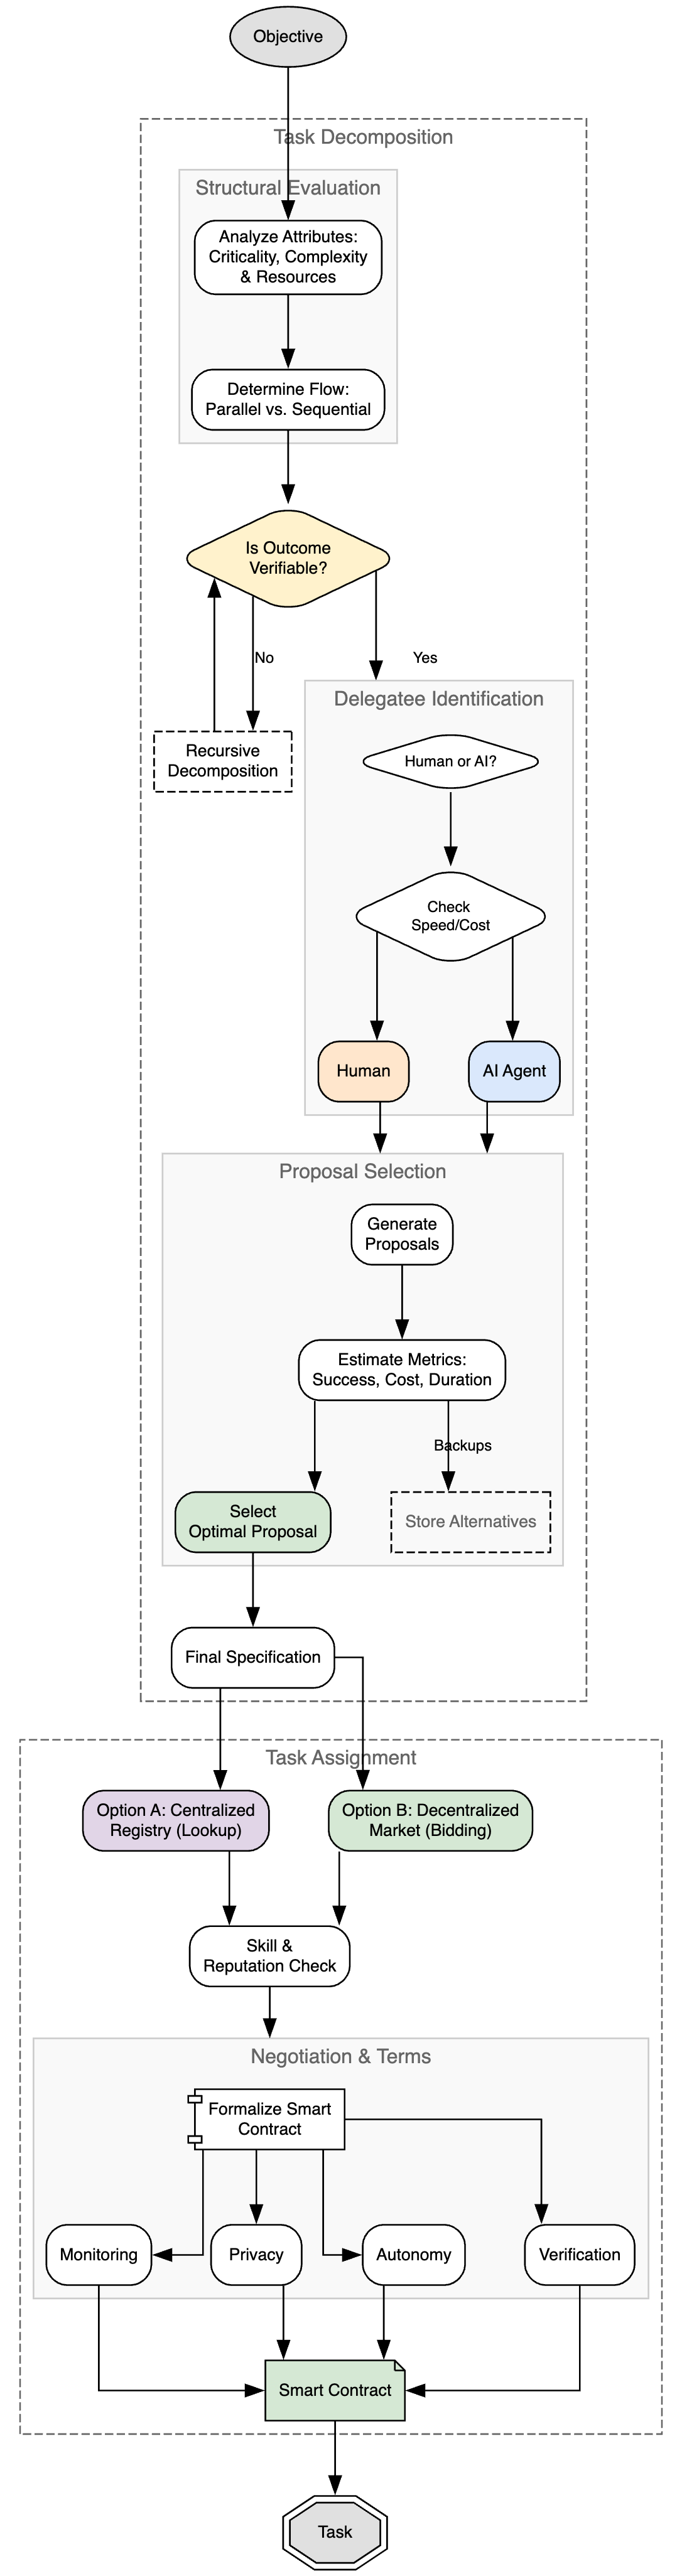
\includegraphics[width=\textwidth, height=0.9\textheight, keepaspectratio]{delegation_flow.png}
    \caption{작업 및 작업의 조작도입니다.}
    \label{fig:pipeline}
\end{figure}

\clearpage
\twocolumn

\subsection{다중 목표최적화}
\label{sec:opt}

지능형 작업 위임의 핵심은 Multi-objective Optimization 문제~\citep{deb2016multi}입니다. delegator는 단일 측정항목을 최적화하려고 하는 경우가 거의 없으며 종종 수많은 경쟁 측정항목 간에 균형을 유지합니다. 가장 효과적인 위임 선택은 가장 빠르거나, 저렴하거나, 가장 정확한 것이 아니라 이러한 요소들 사이에서 최적의 균형을 유지하는 것입니다. 최적이라고 간주되는 것은 상황에 따라 다르며 delegator의 특정 제약 조건 및 선호도에 맞춰 조정되고 전체 리소스 가용성에 맞춰 조정되어야 합니다.

최적화 환경은 \ref{sec:foundations} 섹션에 정의된 작업 특성에 직접 매핑되는 경쟁 목표로 구성되어 있으며 비용, 불확실성, 개인 정보 보호, 품질 및 효율성의 복잡한 균형이 필요합니다. 고성능 에이전트는 일반적으로 더 높은 수수료를 요구하고 종종 광범위한 계산 리소스가 필요하므로 출력 품질과 운영 비용 사이에 긴장이 생깁니다. 반대로, 리소스 소비를 줄이면 실행 속도가 느려지는 경우가 많아 대기 시간과 비용 간에 직접적인 균형이 이루어집니다. 불확실성은 지출과 유사하게 결합됩니다. 평판이 좋은 에이전트나 프리미엄 데이터 액세스 도구를 활용하면 위험은 줄어들지만 비용은 증가하는 반면, 비용 최소화 전략은 본질적으로 실패 확률을 높입니다. 개인 정보 보호 제약으로 인해 더욱 복잡해졌습니다. 성능을 극대화하려면 완전한 컨텍스트 투명성이 필요한 경우가 많지만, 데이터 난독화 또는 동형 암호화와 같은 개인 정보 보호 기술은 상당한 계산 오버헤드를 발생시킵니다. 결과적으로 delegator는 \textit{신뢰-효율의 경계}를 탐색하여 컨텍스트 누출 및 검증 예산에 대한 엄격한 제약을 충족시키면서 성공 확률을 최대화하려고 합니다. 마지막으로, 목적 함수는 인간 기술 보존과 같은 보다 광범위한 사회적 목표를 포함하도록 확장될 수 있습니다(Section~\ref{sec:deskill}).

Multi-objective Optimization 측면에서 delegator는 선택한 솔루션이 달성 가능한 다른 옵션에 의해 지배되지 않도록 하기 위해 파레토 최적성을 추구합니다. 복잡한 제약 조건과 절충안을 통합하려면 정량적 제안 지표를 보완하기 위한 공개 협상이 필요한 경우가 많습니다. 최적화 프로세스는 초기 위임 시 수행되는 일회성 이벤트가 아닙니다. 이는 연속 루프로 실행되어 monitoring 신호를 실제 성능 데이터의 스트림으로 통합하고 각 에이전트의 성공 가능성, 예상 작업 기간 및 비용에 대한 delegator의 믿음을 업데이트합니다. 실행 시 상당한 드리프트(임시 식별된 대체 솔루션에 비해 최적성 격차 발생)로 인해 재최적화 및 재할당이 발생합니다. 실행 중에 전환할 때 오버헤드와 리소스 낭비가 발생하므로 이러한 결정에는 적응 비용도 포함되어야 합니다.

delegator는 delegator의 추론 제어 흐름에 대한 계산 비용과 함께 협상, 계약 생성 및 검증의 총 비용인 전체 \emph{위임 타워 헤드}도 고려해야 합니다. 결과적으로, 낮은 중요성, 높은 확실성 및 짧은 기간을 특징으로 하는 작업이 직접 실행을 위해 intelligent delegation protocol을 우회할 수 있는 복잡성 수준이 설정됩니다. 그렇지 않으면 거래 비용이 업무 가치를 초과하여 업무 위임이 불가능해질 수 있습니다.

\subsection{적응형 조정}
\label{sec:adapt}

\begin{figure*}[t]
    \centering
    \makebox[\textwidth][c]{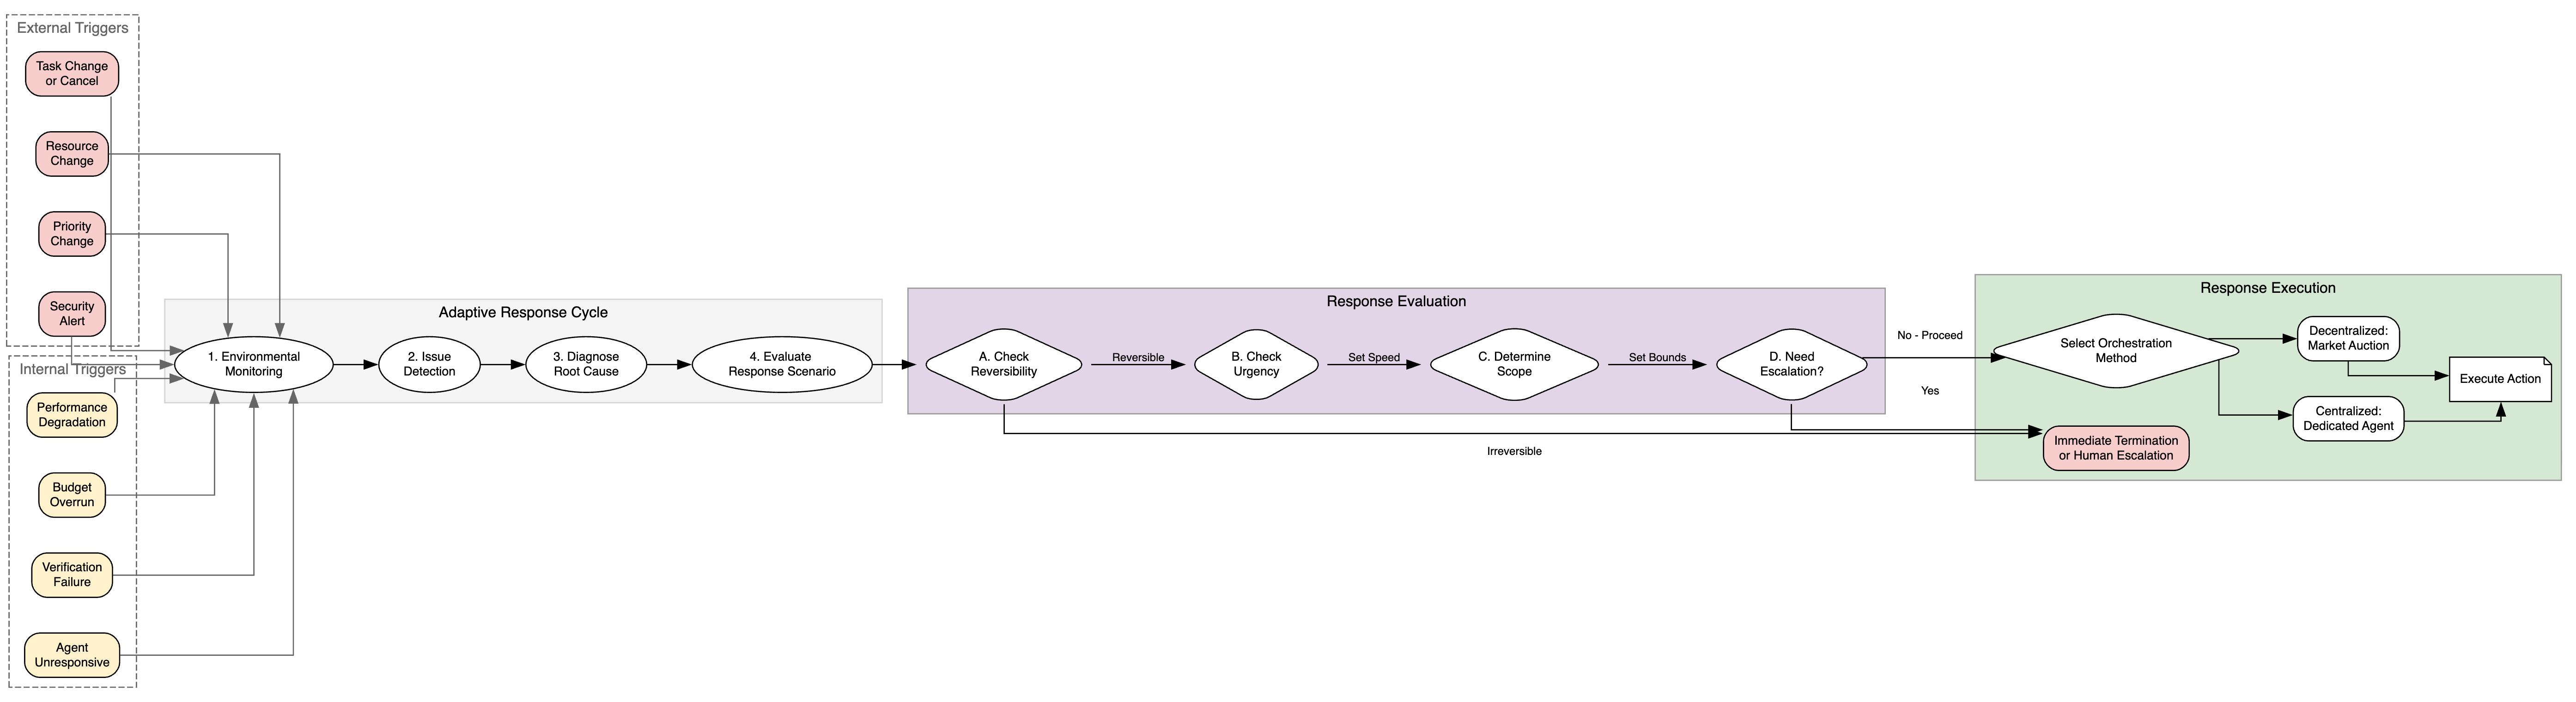
\includegraphics[width=1.2\textwidth, height = 8cm]{coordination.png}}
    \caption{적응 조정주기. 다양한 유형의 환경 때문에 그럴 수 있도록 설정이 동적으로 재평가되어 변경될 수 있습니다.}
    \label{fig:coordination}
\end{figure*}

불확실성이 높거나 기간이 긴 작업의 경우 정적 실행 계획으로는 충분하지 않습니다. 매우 동적이고 개방적이며 불확실한 환경에서 이러한 작업을 위임하려면 \emph{적응적}이 필요하며 고정적이고 정적인 실행 계획에서 벗어납니다. task assignment은 \emph{외부} 또는 \emph{내부} 트리거에서 발생할 수 있는 런타임 우발 상황에 응답해야 합니다. 이러한 변화는 관련 상황 정보의 흐름을 포함하여 monitoring(\ref{sec:monitor} 섹션 참조)을 통해 식별됩니다.

delegator가 적응하고 재위임하게 만드는 외부 요인은 여러 가지가 있습니다. 첫째, delegator는 작업 사양을 변경하거나 목표를 변경하거나 추가 제약 조건을 도입할 수 있습니다. 둘째, 작업이 취소될 수 있습니다. 셋째, 외부 자원의 가용성이나 비용에 변화가 발생할 수 있습니다. 예를 들어 중요한 타사 API가 중단되거나, 데이터세트에 액세스할 수 없게 되거나, 컴퓨팅 비용이 급증할 수 있습니다. 넷째, 현재 작업보다 우선순위가 높은 새 작업이 대기열에 들어갈 수 있으므로 우선순위가 낮은 작업에 사용되는 리소스를 선점해야 합니다. 마지막으로, 보안 시스템은 delegator의 잠재적으로 악의적이거나 유해한 행동을 식별하여 즉각적인 종료가 필요할 수 있습니다.

내부 요인의 경우 delegator가 원래 위임 전략을 채택하기로 결정하는 데에는 몇 가지 이유가 있습니다. 첫째, 특정 delegator는 성능 저하를 경험하여 처리 대기 시간, 처리량 또는 진행 속도와 같이 합의된 서비스 수준 목표를 충족하지 못할 수 있습니다. 둘째, delegator는 할당된 예산을 초과하여 리소스를 소비하거나 작업을 효과적으로 완료하기 위해 리소스 증가가 필요하다고 판단할 수 있습니다.\footnote{복잡한 환경에서는 정확한 예산 추정이 어렵기 때문에 이 시나리오는 자주 나타날 것으로 예상할 수 있습니다.} 셋째, delegator가 생성한 중간 아티팩트가 확인 검사에 실패할 수 있습니다. 마지막으로 특정 agent이 응답하지 않아 추가 요청을 승인하지 못할 수도 있습니다.

트리거를 식별하면 적응형 응답 주기가 시작되어 전체 위임 체인에 걸쳐 시정 조치가 조정됩니다. 이 프로세스는 문제를 식별하기 위해 대표자와 환경을 지속적으로 monitoring하는 것으로 시작됩니다. 문제가 감지되면 delegator는 근본 원인을 진단하고 잠재적인 대응 시나리오를 평가하여 선택합니다. 이 평가에는 대응이 얼마나 빨라야 하는지 설정하는 것이 포함됩니다. 덜 긴급한 상황에서는 delegator에게 재위임할 시간이 더 많이 주어지는 반면, 긴급한 상황에서는 즉각적이고 계획적인 대응이 필요합니다. 응답 범위는 다양할 수 있습니다. 운영 매개변수를 조정하거나 하위 작업을 다시 위임하거나 task decomposition를 완전히 다시 실행하고 새로 파생된 여러 하위 작업을 재할당하는 것만큼 독립적입니다. 문제는 위임 체인을 통해 원래 delegator나 인간 감독자에게 에스컬레이션되어야 할 수도 있습니다. 대응 시나리오의 선택은 궁극적으로 작업의 가역성에 따라 결정됩니다. 되돌릴 수 있는 하위 작업 오류는 자동 재위임을 트리거할 수 있는 반면, 되돌릴 수 없고 중요도가 높은 작업의 오류는 즉시 종료되거나 인적 에스컬레이션을 트리거해야 합니다.

응답 오케스트레이션은 위임 네트워크의 중앙 집중화 수준에 따라 달라집니다. 중앙화된 경우에는 전담 delegator가 책임을 집니다. 이 에이전트는 위임된 작업, delegator 기능 및 진행 상황에 대한 전체적인 보기를 유지합니다. 트리거가 감지되면 에이전트는 작업 취소 요청을 발행하고 새 delegator에게 다시 위임합니다. 중앙 집중식 시스템의 단점은 단일 실패 지점이 발생하기 때문에 취약할 수 있다는 것입니다. 중앙 집중식 오케스트레이터는 제어 계산 범위(Section~\ref{sec:human})에 의해 근본적으로 제한됩니다. 인간 관리자가 인지적 한계에 직면하는 것처럼 중앙 집중식 의사결정 노드도 병목 현상을 유발하는 대기 시간 및 계산 한계에 직면할 수 있습니다. 

시장 기반 메커니즘을 통한 분산형 조정이 대안을 제공합니다. 여기서 새로 파생된 위임 요청은 위임 후보 에이전트가 입찰할 수 있도록 경매 대기열에 푸시될 수 있습니다. agent이 작업을 불이행하고 해당 작업이 다시 경매되는 경우, 불이행 agent은 벌금으로 가격 차액을 충당해야 할 수도 있습니다. 단일 입찰에서 적합성이 쉽게 표현되지 않는 복잡한 작업의 경우 에이전트는 다단계 협상에 참여할 수 있습니다. 스마트 계약으로 인코딩된 위임 계약에는 적응형 조정을 위해 사전 합의된 실행 조항이 포함될 수도 있습니다. 예를 들어, 위임 계약의 조항은 백업 에이전트, 작업을 자동으로 재할당하는 기능 및 기본 delegator가 지정된 기한까지 유효한 영지식 증명 체크포인트를 제출하지 못할 경우 백업에 대한 관련 지불을 지정할 수 있습니다.

적응형 작업 재할당 메커니즘은 시장 수준의 안정성 조치와 결합되어야 합니다. 그렇지 않으면 일련의 이벤트가 과도한 트리거로 인해 불안정해질 수 있습니다. 예를 들어, 약간의 자격을 갖춘 대표자 간에 작업이 앞뒤로 전달되어 바람직하지 않은 변동이 발생할 수 있습니다. 단일 실패로 인해 리소스가 매우 비효율적이거나 시장을 압도하는 일련의 재할당이 발생할 수도 있습니다. 따라서 재입찰의 휴지 기간을 보장하거나 평판 업데이트의 저하 요인을 보장하거나 빈번한 재위임에 대한 수수료를 인상하는 특별한 조치가 있을 수 있습니다.

\subsection{monitoring}
\label{sec:monitor}

\begin{table*}[t]
\caption{지능형 분석의 검토 방식을 결정합니다.}
\label{tab:monitoring_taxonomy}
\centering
\begin{tabular}{@{}lp{6.5cm}p{6.5cm}@{}}
\toprule
\textbf{차원} & \textbf{옵션 A(경량)} & \textbf{옵션 B(집중)} \\ \midrule
\textbf{목표} 및 \textbf{결과 범주}: 최종 결과의 사후 검증(예: 바이너리 성공 플래그, 품질 점수). & \textbf{프로세스 수준}: 중간 상태, 리소스 소비 및 방법론을 지속적으로 추적합니다. \\ \midrule
\textbf{관찰 가능성} & \textbf{간접}: 환경적 부작용(예: 파일 시스템 변경)을 통해 진행 상황을 추론합니다. & \textbf{직접}: 명시적 상태 폴링, 푸시 알림 또는 실시간 이벤트 스트리밍 API. \\ \midrule
\textbf{투명도} & \textbf{블랙박스}: 입력/출력 관찰 전용; 내부 상태는 숨겨진 상태로 유지됩니다. & \textbf{화이트박스}: 내부 추론 추적, 결정 논리 및 메모리에 대한 전체 검사. \\ \midrule
\textbf{은둔} & \textbf{완전한 숫자}: delegator는 delegator에게 데이터와 중간 아티팩트를 공개합니다. & \textbf{암호화}: 데이터를 공개하지 않고 정확성을 확인하는 영지식 증명(zk-SNARKs) 또는 MPC. \\ \midrule
\textbf{토폴로지} & \textbf{직접}: 직속 agent만 monitoring합니다(1:1). & \textbf{전이적}: 하위 agent을 확인하기 위해 중간 에이전트의 서명된 증명에 의존합니다. \\ \bottomrule
\end{tabular}
\end{table*}

작업 위임의 맥락에서 monitoring은 위임된 작업의 상태, 진행 상황 및 결과를 관찰, 측정 및 확인하는 체계적인 프로세스입니다. 따라서 이는 계약 준수 보장, 오류 감지, 실시간 개입 활성화, 후속 성능 평가를 위한 데이터 수집, 평판 시스템 기반 구축 등 몇 가지 중요한 기능을 수행합니다. monitoring 구현은 여러 축에 걸쳐 세분화될 수 있으므로(표 \ref{tab:monitoring_taxonomy} 참조) 강력한 monitoring 시스템은 더 가볍거나 집중적일 수 있는 여러 보완 솔루션을 통합해야 합니다.

첫 번째 축은 monitoring 대상입니다. \emph{결과 범위 monitoring}은 에이전트 작업의 최종 결과에 중점을 둡니다. 이 사후 확인은 작업이 성공적으로 완료되었는지 여부를 나타내는 이진 플래그, 정량적 척도(예: 1-10) 또는 delegator 또는 신뢰할 수 있는 제3자가 제공한 정성적 feedback일 수 있습니다. 반면 \emph{프로세스 수준 monitoring}은 중간 상태, 리소스 소비 및 delegator가 사용하는 방법론을 추적하여 작업 자체의 실행에 대한 지속적인 통찰력을 제공합니다. 보다 리소스 집약적인 프로세스 수준 monitoring인 반면~\citep{lightman2023letsverifystepstep}는 장기 실행, 중요 또는 \emph{어떻게}가 \emph{무엇}만큼 중요한 작업에 필수적입니다. 이는 안전을 보장하기 위해 읽기 쉬운 중간 추론 단계의 검사가 필요할 수 있는 확장 가능한 감독(\citep{bowman2022measuringprogressscalableoversight, saunders2022selfcritiquingmodelsassistinghuman})의 기초를 형성합니다.

두 번째 축은 관찰 가능성입니다. monitoring은 직접적이거나 간접적일 수 있습니다. 직접 monitoring에는 delegator가 delegator에게 상태 업데이트를 쿼리하는 명시적인 통신 protocol이 포함됩니다. 반면, 간접 monitoring은 직접적인 의사소통 없이 공유된 환경 내에서 delegator의 행동이 미치는 영향을 관찰하여 진행 상황을 추론하는 것입니다. 예를 들어 delegator는 공유 파일 시스템, 데이터베이스 또는 버전 제어 저장소에서 진행 상황을 나타내는 변경 사항을 monitoring할 수 있습니다. 이 프로세스는 덜 방해적이지만 덜 정확할 수도 있고 환경을 완전히 관찰할 수 없는 경우 실행 가능성도 낮을 수도 있습니다.

이러한 접근 방식은 기술적인 관점에서 다양한 방식으로 실현될 수 있습니다. 직접 monitoring의 가장 간단한 구현은 잘 정의된 API에 의존합니다. delegator는 주기적으로 GET /task/{id}/status 엔드포인트를 폴링하거나 푸시 기반 알림을 위한 웹후크를 구독할 수 있습니다. 보다 세분화된 실시간 프로세스 monitoring을 위해 Apache Kafka 또는 gRPC 스트림과 같은 이벤트 스트리밍 플랫폼을 사용할 수 있습니다. delegator 에이전트는 delegator가 나중에 검사할 수 있는 TASK\_STARTED, CHECKPOINT\_REACHED, RESOURCE\_WARNING 및 TASK\_COMPLETED와 같은 이벤트를 게시할 수 있습니다. 표준화된 관찰 protocol의 개발은 agentic web~\citep{blanco2023practical}의 상호 운용성을 보장하는 데 중요합니다. 블록체인의 스마트 계약을 사용하면 위임 에이전트가 주요 진행 상황이나 체크포인트를 블록체인에 게시하도록 할 수 있습니다. 이는 성능 저하에 대한 응답으로 알고리즘 트리거에 의해 결합되어 monitoring 프로세스에 수반되는 \emph{알고리즘} 수준으로 이어질 수 있습니다.

세 번째 축은 시스템 투명성이다. \emph{블랙박스 monitoring}에서는 위임 agent을 봉인된 단위로 취급합니다. delegator는 입력과 출력, 그리고 해당 작업의 직접적인 결과만 관찰할 수 있습니다. 이는 delegator가 독점 모델이거나 타사 서비스인 경우에 일반적입니다. \emph{화이트박스} monitoring은 delegator에게 delegator의 내부 상태, 추론 프로세스 또는 결정 논리에 대한 액세스 권한을 부여합니다. 이는 고급 AI 에이전트의 디버깅, 감사 및 정렬을 보장하는 데 중요합니다. delegator가 사람인 경우 완전한 블랙박스 monitoring은 기술적으로 불가능하지만 의도, 추론, 정당성을 요구하여 균형을 맞추는 것은 가능할 수 있습니다. 강력한 블랙박스 monitoring protocol은 생성된 모델의 자연어 생각이 모델의 실제 내부 상태(\citep{turpin2023languagemodelsdontsay})와 항상 충실하게 일치하지 않는다는 사실도 고려해야 합니다.

네 번째 축은 개인 정보 보호입니다. 위임된 작업이 개인 데이터, 민감한 데이터 또는 독점 데이터와 관련된 경우 심각한 문제가 발생합니다. delegator는 진행 상황과 정확성에 대한 보증을 요구하지만, delegator는 원시 데이터나 중간 계산 결과물을 공개하는 것이 제한될 수 있습니다. 데이터 민감도가 낮은 시나리오에서 가장 효율적인 솔루션은 \emph{완전한 숫자}입니다. 여기서 delegator는 단순히 모든 데이터와 중간 아티팩트를 delegator에게 공개합니다. 그러나 이러한 접근 방식은 GDPR 또는 HIPAA와 같은 규정이 적용되는 민감한 영역이나 delegator의 중간 통찰력이 영업 비밀을 구성하는 영역에서는 종종 지원되지 않습니다. 이러한 경우 운영 방법을 공개하면 delegator의 시장 지위가 손상되거나 내부 상태가 악용에 노출되어 보안 취약점이 발생할 수 있습니다. 이러한 제약 속에서 안전하게 monitoring을 구현하려면 고급 암호화 기술을 활용하는 것이 필요합니다. 영지식 증명을 사용하면 delegator('증명자')가 delegator('검증자')에게 데이터 자체를 공개하지 않고도 데이터세트에서 계산이 올바르게 수행되었음을 입증할 수 있습니다. 예를 들어, 민감한 데이터 세트를 분석하는 임무를 맡은 에이전트는 결과의 특정 속성을 증명하는 간결한 비대화형 지식 인수(zk-SNARK)~\citep{bitansky2013succinct, petkus2019and}를 생성할 수 있습니다. delegator는 이 증거를 즉시 확인하여 기본 민감한 데이터를 보지 않고도 결과의 확실성을 얻을 수 있습니다. 또는 동형암호 \citep{acar2018survey} 및 보안 다자간 계산 \citep{goldreich1998secure, knott2021crypten}를 사용하면 암호화된 데이터에 대해 계산을 수행할 수 있습니다. 이러한 방법은 작업 실행 및 monitoring에 모두 적용됩니다. delegator는 암호화된 중간 상태에 대해 사전 동의된 monitoring 기능을 수행하고 그 결과를 delegator에게 보냅니다. delegator는 규정 준수 여부를 확인하기 위해 암호를 해독할 수 있는 유일한 당사자입니다.

마지막 축은 토폴로지입니다. agentic web에서 발생할 수 있는 복잡한 네트워크 전체에서 작업을 분해하고 다시 위임하여 위임 체인을 형성할 수 있습니다. 에이전트 $A$는 $B$에 위임하고 작업의 일부를 $C$에 하위 위임하는 식입니다. 이는 효과적인 \emph{전이적 모델링}을 달성하는 문제를 소개합니다. 이러한 위임 체인에서는 원래 delegator(위 예에서는 에이전트 $A$)가 에이전트 $C$를 직접 monitoring하거나 $B$를 monitoring하는 것과 동일한 정도로 $C$를 monitoring하는 것이 불가능할 수 있습니다. $A$는 $B$와 스마트 위임 계약을 맺을 수 있고 $B$는 $C$와 계약을 맺을 수 있지만 $A$도 $C$와 계약하지 않는 한 해당 조항은 적용되지 않을 수 있습니다. 다른 이유로 인해 $B$는 공급자($C$)를 클라이언트($A$)에 노출시키지 않을 수 있습니다. 기술적으로 $A$, $B$ 및 $C$는 서로 다른 monitoring protocol을 사용할 수 있으며 네트워크 내 각 에이전트의 평판 차이로 인해 서로 다른 monitoring 수준에 동의할 수 있습니다. 각 개별 위임 링크마다 개인정보 보호 문제가 있을 수 있습니다. 따라서 보다 실용적인 모델은 \emph{증명을 전이적 책임}입니다. 이 프레임워크에서 에이전트 $B$는 agent $C$를 monitoring합니다. 그런 다음 $B$는 $C$ 성능에 대한 요약 보고서를 생성합니다(예: ``하위 작업\_2 완료, 품질 점수: 0.87, 소비된 리소스: 5 GPU 시간''). 그런 다음 $B$는 보고서에 암호화 방식으로 서명하고 이를 자체 예약 상태 업데이트에 포함된 $A$로 전달합니다. 에이전트 $A$는 $C$를 직접 monitoring하지 않고 대신 $B$의 $C$ monitoring 기능을 monitoring합니다. 이러한 위임된 monitoring이 효과적이려면 $A$가 $B$의 검증 기능을 신뢰할 수 있어야 하며, 이는 $B$가 신뢰할 수 있는 제3자에 의해 인증된 monitoring 프로세스를 보유함으로써 보장될 수 있습니다.

\subsection{신뢰와 평판}
\label{sec:trust}

\begin{table*}[t]
\caption{평판 구현에 대한 방식.}
\label{tab:reputation_approaches}
\centering
\begin{tabular*}{\textwidth}{@{\extracolsep{\fill}}lp{0.35\textwidth}p{0.35\textwidth}@{}}
\toprule
\textbf{평판 모델} & \textbf{기구} & \textbf{공익사업} \\ \midrule
\textbf{불변의 원장} & 작업 결과, 리소스 소비 및 제약 준수를 변조 방지 블록체인에서 검증 가능한 트랜잭션으로 인코딩합니다. & 위험도가 낮은 작업 선택을 통해 '게임'에 대한 보호 장치가 필요하지만 소급 변조를 방지하는 기본 성능 기록을 확립합니다. \\ \midrule
\textbf{신뢰의 웹} 및 분산형 식별자를 활용하여 특정 기능을 증명하는 서명된 상황별 검증 가능한 자격 증명을 발급합니다. & 일반적인 점수를 넘어 포트폴리오 모델로 이동하여 도메인별 전문 지식과 신뢰할 수 있는 제3자 보증을 기반으로 정확한 위임을 가능하게 합니다. \\ \midrule
\textbf{행동 지표} 및 실행 프로세스, 특히 추론 추적 및 protocol 준수의 명확성을 분석하여 투명성과 안전 점수를 도출합니다. & \emph{어떻게} 결과가 아닌 작업이 수행되어 고위험 작업이 안전 표준에 부합하는지 확인합니다. \\ \bottomrule
\end{tabular*}
\end{table*}

신뢰 및 평판 메커니즘은 확장 가능한 위임의 기반을 구성하여 트랜잭션 마찰을 최소화하고 개방형 multi-agent 환경에서 안전성을 향상시킵니다. 우리는 신뢰를 명시적인 제약 조건과 암묵적인 의도에 따라 작업을 실행하는 delegator의 능력에 대한 delegator의 믿음 정도로 정의합니다. 이러한 믿음은 이전에 설명한 monitoring protocol을 통해 수집된 검증 가능한 데이터 스트림을 기반으로 동적으로 형성되고 업데이트됩니다(\ref{sec:monitor} 섹션 참조). 

평판은 집계되고 검증 가능한 과거 행동 내역에서 파생된 예측 신호 역할을 하며 에이전트의 잠재적 신뢰성과 정렬을 나타내는 프록시 역할을 합니다. 우리는 평판을 에이전트의 신뢰성에 대한 공개적이고 검증 가능한 기록으로 구분하고, 신뢰를 delegator가 설정한 개인적이고 상황에 따른 임계값으로 구분합니다. 에이전트는 전반적인 평판이 높지만 특정 고위험 작업에 필요한 특정 상황별 신뢰 임계값을 충족하지 못할 수 있습니다. 신뢰와 평판을 통해 delegator는 delegator를 선택할 때 정보에 입각한 결정을 내릴 수 있으며, agent에게 부여된 자율성과 감독 수준을 효과적으로 관리할 수 있습니다. 신뢰도가 높을수록 delegator는 monitoring 및 검증 비용을 절감할 수 있습니다.

평판 메커니즘은 다양한 방식으로 구현될 수 있습니다(표 \ref{tab:reputation_approaches} 참조). 가장 직접적인 접근 방식은 이를 성능 기반 불변 원장으로 인코딩하는 것입니다. 여기서 완료된 각 작업은 작업 완료 성공 또는 실패, 총 리소스 소비(컴퓨팅, 시간), 마감일 준수, 제약 조건 준수, delegator가 판단한 최종 출력 품질 등 검증 가능한 지표가 포함된 트랜잭션으로 기록됩니다. 원장의 불변성은 에이전트의 기록을 조작하는 것을 방지하여 평판에 대한 신뢰할 수 있는 기반을 제공합니다. 그러나 순진한 구현은 게임에 취약할 수 있습니다. 예를 들어 에이전트는 단순하고 위험도가 낮은 작업만 수락하여 평판을 부풀릴 수 있습니다. 이러한 제한은 분산형 증명 및 \emph{신뢰의 웹} 모델에 의존하고 분산형 식별자 및 검증 가능한 자격 증명과 같은 기술을 활용하여 극복할 수 있습니다. 이 모델에서 평판은 단일 점수가 아니라 다른 에이전트가 발급한 서명된 상황별 자격 증명의 포트폴리오로 구상됩니다. delegator와 작업을 일치시키려는 경우 delegator는 평판이 좋은 AI 컨소시엄에서 발행한 특정 기술이나 도메인(예: 법률 문서 번역 서비스)을 증명하는 검증 가능한 자격 증명을 보유한 에이전트에 대한 쿼리를 발행할 수 있습니다. 마지막 접근 방식은 행동 및 설명 가능성 지표에 더 초점을 맞추는 것입니다. 여기서 평판은 최종 결과뿐만 아니라 에이전트가 작업을 수행하는 방식에 따라 달라집니다. 다른 평판 메커니즘을 보완하기 위해 \emph{투명성 점수}를 포함하는 것이 가능할 것입니다. 이 점수는 제공된 추론 및 설명의 명확성과 건전성뿐만 아니라 사전 정의된 안전 protocol 준수에서 파생된 \emph{안전 점수}에 대한 정보를 제공합니다.

평판 지표의 역할은 전체 작업 위임 수명 주기에 걸쳐 확장됩니다. 초기 매칭 단계에서 평판 점수는 delegator 필터링 메커니즘의 역할을 할 수 있습니다. 더욱이 신뢰는 권위와 자율성의 역동적인 범위를 알려줍니다. 이러한 등급화된 권한 메커니즘으로 인해 신뢰도가 낮은 에이전트는 거래 가치 한도 및 필수 감독과 같은 엄격한 제약에 직면하게 되고, 평판이 높은 에이전트는 최소한의 개입으로 작동하게 됩니다. 이 동적 교정은 계산 가능한 신뢰를 활용하여 운영 효율성과 안전 간의 균형을 최적화합니다. 평판 자체는 귀중한 무형 자산이 되어 에이전트가 신뢰할 수 있고 진실되게 행동할 수 있도록 강력한 경제적 인센티브를 제공합니다. 평판이 손상되면 향후 수익 잠재력이 제한되기 때문입니다.

또한 신뢰 프레임워크는 인간 참여자를 보편적으로 수용해야 합니다. 이를 위해서는 인간 사용자가 계산적으로 에이전트 평판을 확인할 수 있는 동시에 agentic web의 사기 및 악의적인 이용을 완화하기 위해 자신의 평판 상태를 유지할 수 있는 도구가 필요합니다. 신뢰할 수 있는 에이전트가 악의적인 인간 지시를 엄격하게 실행하여 불공정한 평판 손상을 초래할 수 있는 경우 심각한 문제가 발생합니다. 이를 완화하기 위해 상담원은 들어오는 요청을 엄격하게 평가하고 필요한 경우 설명이나 추가 컨텍스트를 요청하거나 적절한 경우 요청을 거부해야 합니다. 또한 시장 감사에서는 에이전트 실행 실패와 악의적인 지시를 구별하여 복잡한 위임 체인 내에서 책임의 정확한 귀속을 보장해야 합니다.

\subsection{Permission Handling}
\label{permission}

AI 에이전트에 자율성을 부여하면 중요한 취약성 표면이 발생합니다. 즉, 행위자가 민감한 리소스를 과도하거나 무한한 위험에 노출시키지 않고 목표를 실행할 수 있는 충분한 권한을 갖도록 보장합니다. Permission Handling는 운영 효율성과 시스템적 안전성 사이의 균형을 유지해야 하며, 저위험 도메인과 고위험 도메인에 대해 다르게 처리되어야 합니다. 표준 데이터 스트림 또는 일반 도구를 포함하는 낮은 중요도 및 높은 가역성(Section~\ref{sec:foundations})을 특징으로 하는 일상적인 저위험 작업의 경우 에이전트에는 조직 멤버십, 활성 안전 인증 또는 신뢰할 수 있는 임계값을 초과하는 평판 점수와 같은 검증 가능한 속성에서 파생된 기본 상시 권한이 부여될 수 있습니다. 이는 마찰을 줄이고 위험도가 낮은 환경에서 자율적인 상호 운용성을 가능하게 합니다. 반대로, 높은 작업 중요성과 상황성을 나타내는 고위험 영역(예: 의료, 중요 인프라)에서는 권한이 위험에 적응해야 합니다. 이러한 시나리오에서는 정적 자격 증명으로는 충분하지 않습니다. 민감한 API 또는 제어 시스템에 대한 액세스는 대신 적시에 부여되고, 즉각적인 작업 기간으로 엄격하게 범위가 지정되며, 필요한 경우 필수 인간 루프 승인 또는 제3자 승인에 의해 제어됩니다. 이러한 엄격한 게이팅은 혼란스러운 agent 문제 \citep{hardy1988confused}를 완화하는 데 필요합니다. 여기서 기술적으로 유효한 자격 증명을 보유하고 있는 손상된 에이전트가 악의적인 외부 행위자 \citep{liu2023prompt} 및 적대적 콘텐츠에 의해 해당 자격 증명을 오용하도록 속일 수 있습니다.

또한 권한 부여 프레임워크는 권한 약화를 통한 작업 위임의 반복적 특성을 설명해야 합니다. 에이전트가 작업을 하위 위임하면 전체 권한 집합을 전송할 수 없습니다. 대신 해당 특정 하위 작업에 필요한 리소스의 엄격한 하위 집합에 대한 액세스를 제한하는 권한을 발급해야 합니다. 이를 통해 네트워크 가장자리에서의 손상이 시스템 침해로 확대되지 않도록 보장합니다. 또한 권한 세분성은 바이너리 액세스 이상으로 확장되어야 합니다. 에이전트는 도구나 데이터 세트뿐만 아니라 허용되는 특정 작업(예: 특정 행에 대한 읽기 전용 액세스 또는 특정 기능에 대한 실행 전용 액세스)에 따라 액세스가 정의되는 의미론적 제약 조건에 따라 작동해야 하며, 의도하지 않은 목적으로 광범위한 기능을 오용하는 것을 방지해야 합니다. 체인의 특정 delegator가 delegator에게 부여할 수 있는 권한을 관리하려면 메타 권한이 필요할 수 있습니다. AI 에이전트는 자신의 능력에 따라 행동할 수 있는 특정 기능 및 관련 권한을 갖고 있는 동시에 다른 에이전트가 충분히 능력이 있거나 신뢰할 수 있는지를 보다 광범위하게 평가할 만큼 지식이 부족할 수 있습니다. 그러한 에이전트가 여전히 작업 하위 위임을 고려하는 경우 제안을 온전하게 확인하고 의도된 권한 전송을 승인할 제3자인 외부 검증자에게 문의해야 할 수도 있습니다.

마지막으로 권한의 수명주기는 지속적인 검증과 자동 취소를 통해 관리되어야 합니다. 액세스 권한은 정적 부여가 아니라 에이전트가 필수 신뢰 지표를 유지하는 동안에만 지속되는 동적 상태입니다. 프레임워크는 알고리즘 회로 차단기를 구현해야 합니다. 에이전트의 평판 점수가 갑자기 떨어지거나(\ref{sec:trust} 섹션 참조) 이상 탐지 시스템이 의심스러운 동작을 표시하는 경우 활성 토큰은 위임 체인 전체에서 즉시 무효화되어야 합니다. 이러한 복잡성을 대규모로 관리하려면 권한 부여 규칙을 코드형 정책을 통해 정의해야 합니다. 이를 통해 조직은 배포 전에 보안 상태를 감사, 버전 지정 및 수학적으로 확인할 수 있으므로 대량의 개별 권한 부여의 총 효과가 시스템의 안전 불변성과 일치하도록 보장할 수 있습니다.

\subsection{검증 가능한 접착제}
\label{sec:verify}

위임 수명주기는 임시 결과를 검증하고 마무리하는 메커니즘인 검증 가능한 작업 완료로 마무리됩니다. 이 프로세스는 프레임워크의 계약상 초석을 구성하여 delegator가 작업을 공식적으로 \emph{닫기}하고 합의된 거래의 합의를 촉발할 수 있게 해줍니다. 검증은 에이전트 시장 내에서 잠정적 결과를 확정된 사실로 변환하고 지불 해제, 평판 업데이트 및 책임 할당을 위한 기반을 설정하는 최종 이벤트 역할을 합니다. 결정적으로, 효과적인 검증은 나중에 고려하는 것이 아니라 설계에 대한 제약입니다. \emph{계약 초기 분해} 원칙(Section~\ref{sec:decomp})에서는 작업 세분성을 \emph{선험적으로} 사용 가능한 검증 기능에 맞게 조정하여 위임된 모든 목표가 본질적으로 검증 가능하도록 보장해야 합니다.

프레임워크 내의 검증 메커니즘은 직접 결과 검사, 신뢰할 수 있는 제3자 감사, 암호화 증명 및 게임 이론적 합의로 크게 분류할 수 있습니다. 첫째, 직접적인 결과 검증은 delegator가 최종 결과를 직접 평가할 수 있는 능력, 도구 및 권한을 보유하고 있을 때, 특히 내재적 검증 가능성이 높고 주관성이 낮은 업무의 경우 가능합니다. 이는 코드 생성과 같은 자동 확인 가능한 도메인 \citep{li2024llms}에 적용됩니다.\footnote{구현된 기능을 확인하는 데 사용할 수 있는 해당 테스트 사례 세트가 있는 경우입니다.} 직접 확인에서는 결과가 충분히 투명하고 사용 가능하며 엄청나게 복잡하지 않아야 합니다. 둘째, delegator에게 이러한 아티팩트에 액세스할 수 있는 전문 지식이나 권한이 부족하고 도구 기반 솔루션이 실행 불가능한 시나리오에서는 검증을 신뢰할 수 있는 제3자에게 아웃소싱할 수 있습니다. 이는 전문 감사 agent, 인증된 인간 전문가 또는 심사관 패널일 수 있습니다. 셋째, 암호화 검증은 개방적이고 잠재적으로 적대적인 환경에서 무신뢰 자동 검증을 위한 추가 옵션을 나타냅니다. 이는 민감한 정보를 반드시 공개하지 않고도 정확성에 대한 수학적 확실성을 제공합니다. delegator는 zk-SNARK와 같은 기술을 통해 특정 출력을 생성하기 위해 특정 입력에서 특정 프로그램이 올바르게 실행되었음을 증명할 수 있습니다. 마지막으로, 게임이론적 메커니즘을 사용하여 결과에 대한 합의를 얻을 수 있습니다. 여러 에이전트가 검증 게임~\citep{teutsch2024scalable}를 플레이할 수 있으며, 보상은 대다수 결과(Schelling 포인트~\citep{pastine2017introducing})를 생성한 사람들에게 분배됩니다. TrueBit~\citep{teutsch2018truebit}와 같은 protocol에서 영감을 받은 이 접근 방식은 경제적 인센티브를 활용하여 부정확하거나 악의적인 결과에 대한 위험을 제거합니다. 이러한 메커니즘은 복잡한 작업에 대한 LLM 기반 검증을 더욱 강력하게 만드는 데 특히 관련이 있을 수 있습니다.

delegator가 하위 작업을 확인된 것으로 표시하면 "A$A$ 에이전트는 $B$가 $D$ 날짜에 $S$ 사양에 따라 $T$ 작업을 성공적으로 완료했음을 증명합니다."를 증명하는 부인할 수 없는 영수증 역할을 하는 암호화로 서명된 검증 가능한 자격 증명을 delegator에게 발급합니다. 그런 다음 이 자격 증명은 $B$의 영구적이고 검증 가능한 로그에 통합됩니다. 시장 내 평판. 스마트 계약은 에스크로에서 지불금을 보유하므로 에이전트 간의 위임을 마무리하는 데 중요한 역할을 합니다. 검증 조항은 delegator 또는 승인된 제3자가 서명한 승인 메시지를 받은 후 자금이 해제되는 조건을 지정합니다. 결제가 실행되면 블록체인에서 불변의 거래가 구성됩니다.

위임 체인 $A \rightarrow B \rightarrow C$에서는 검증과 책임이 반복적으로 발생합니다. 에이전트 $A$는 $C$와 직접적인 계약 관계가 없습니다. 따라서 $A$는 $C$에 대한 책임을 직접 확인하거나 물을 수 없습니다. 검증 부담과 책임 가정은 체인 위로 흘러갑니다. 에이전트 $B$는 $C$가 완료한 하위 작업을 확인하는 역할을 담당합니다. 검증에 성공하면 $B$는 $C$로부터 증거를 얻습니다. 그런 다음 $B$는 할당된 작업을 완료하기 위해 $C$의 결과를 자체 workflow에 통합합니다. $B$는 최종 아티팩트를 $A$에 제출할 때 전체 증명 체인도 제출합니다. 따라서 $A$의 검증 프로세스에는 두 단계가 포함됩니다. 1) $B$가 직접 수행한 작업을 검증합니다. 2) $B$가 제공하는 $C$의 서명된 증명을 확인하여 $B$가 자체 하위 agent $C$의 작업을 올바르게 검증했는지 확인합니다. 더 긴 위임 체인 또는 트리형 위임 네트워크에는 여러 검증 단계에 걸쳐 유사한 재귀적 접근 방식이 필요합니다. 위임 체인의 책임은 전이적이며 개별 지점을 따릅니다. agent은 자신에게 부여된 업무 전체에 대해 책임을 지며, 하청업체를 비난함으로써 책임을 면할 수 없습니다. 책임은 계약 체인에서 파생됩니다. 예를 들어, $A$가 $C$의 작업으로 인한 오류로 인해 손실을 입은 경우 $A$는 직접 합의에 따라 $B$에 책임을 집니다. $B$는 계약에 따라 $C$로부터 상환권을 구합니다.

그러나 검증 프로세스에는 오류가 없는 것은 아닙니다. 주관적인 작업~\citep{gunjal2025rubrics}는 정확한 기준표를 사용하더라도 불일치로 이어질 수 있으며 작업이 완료로 표시된 후에야 오류가 발견될 수 있습니다. 특히 주관성이 높고 본질적인 검증 가능성이 낮은 시장에서 이 문제를 해결하기 위해 프레임워크는 스마트 계약에 기반을 둔 강력한 분쟁 해결 메커니즘에 의존합니다. 이러한 계약에는 본질적으로 \emph{중재 조항} 및 \emph{에스크로 억압}이 포함되어야 합니다. 암호경제적 보안을 통해 신뢰를 운용하려면 delegator는 합리적인 준수를 보장하기 위해 실행 전에 에스크로에 금융 지분을 게시해야 합니다. 작업 흐름은 \emph{낙관적인} 모델을 따릅니다. 즉, delegator가 미리 정의된 분쟁 기간 내에 일치하는 채권을 게시하여 공식적으로 이의를 제기하지 않는 한 작업은 성공한 것으로 간주됩니다. 문제가 발생하고 알고리즘 해결이 실패하는 경우 분쟁은 인간 전문가 또는 AI 에이전트로 구성된 분산형 판결 패널에 전달됩니다. 패널의 판결은 에스크로된 자금의 해제 또는 삭감을 촉발하기 위해 스마트 계약으로 다시 feedback됩니다. 마지막으로 분쟁 기간이 아니더라도 사후 오류 발견을 통해 delegator의 평판 점수에 대한 소급 업데이트가 트리거됩니다. 이는 현재 재정적 의무가 없는 경우에도 책임 agent이 오류를 수정하려는 인센티브를 유지하여 시장 내에서 장기적인 가치를 보호합니다.

\subsection{보안}
\label{sec:security}

작업 위임 시 안전을 보장하는 것은 실행 가능성과 채택을 위한 어려운 전제 조건입니다. 격리된 컴퓨팅 도구에서 상호 연결된 자율 에이전트로의 전환은 근본적으로 보안 환경 \citep{tomavsev2025distributional}를 재구성합니다. 지능형 작업 위임 에코시스템에서는 각 단계와 구성 요소를 개별적으로 보호해야 하지만, 전체 공격 표면은 새로운 multi-agent 역학으로 인해 개별 구성 요소의 표면을 능가하므로 연속적인 오류가 발생할 위험이 있습니다. 이러한 보안 환경은 진화하는 계약과 다양한 투명성의 정보 흐름에 따라 관리되는 인간과 AI 행위자 간의 복잡한 상호 작용에 의해 형성됩니다. 

보안 위협은 위임 체인의 양쪽 끝에 있는 적대 행위자와 더 넓은 생태계에 내재된 시스템적 취약점을 구별하여 공격 벡터의 위치에 따라 분류됩니다.

\begin{itemize}
    \item \textbf{악의적 등록}: 해를 끼칠 의도로 작업을 수락하는 에이전트 또는 인간.
    \begin{itemize}
    \item \textbf{데이터 절차}: delegator는 개인 또는 독점 데이터 \citep{lal2022data}를 포함할 수 있는 작업을 위해 제공된 민감한 데이터를 훔칩니다.
    \item \textbf{데이터 해설}: delegator는 예약된 monitoring 업데이트 또는 최종 아티팩트 \citep{cina2023wild}에서 미묘하게 손상된 데이터를 반환하여 delegator의 목표를 훼손하는 것을 목표로 합니다.
    \item \textbf{검증 전복}: delegator는 작업 완료 확인 \citep{liu2023prompt}에 사용되는 AI 비평가를 탈옥하는 것을 목표로 프롬프트 주입 또는 기타 관련 방법을 활용합니다.
    \item \textbf{자원 고갈}: delegator가 의도적으로 과도한 계산 또는 물리적 리소스를 소비하거나 공유 API \citep{de2023distributed}를 압도하여 서비스 거부 공격에 참여합니다.
    \item \textbf{무단 액세스}: delegator는 네트워크 내에서 \citep{or2019dynamic}를 받지 못했을 권한과 권한을 얻기 위해 악성코드를 활용합니다.
    \item \textbf{백도어 구성}: delegator는 작업을 성공적으로 완료하지만 생성된 아티팩트 내에 숨겨진 트리거 또는 취약점을 추가로 포함합니다. 이 취약점은 나중에 delegator 자신이나 제3자가 이용할 수 있습니다~\citep{wang2024badagentinsertingactivatingbackdoor, rando2024universaljailbreakbackdoorspoisoned}. 성능을 저하시키는 데이터 중독과 달리 백도어는 즉각적인 작업 유용성을 유지하여 식별을 회피하는 동시에 향후 보안을 손상시킵니다.

    \end{itemize}
    \item \textbf{악의적 입장자}: 악의적이거나 불법적인 목적을 가지고 작업을 위임하는 agent 또는 인간.
    \begin{itemize}
    \item \textbf{유해 처리받은 내용}: delegator가 불법적이거나 비윤리적이거나 \cite{ashton2022corrupting, blauth2022artificial}에 해를 끼치도록 고안된 업무를 위임했습니다.
    \item \textbf{취약점 조사}: delegator는 위임 에이전트의 능력, 보안 제어 및 잠재적인 약점 \citep{greshake2023not}를 조사하도록 설계된 양성으로 보이는 작업을 위임합니다.
    \item \textbf{신속한 강도 및 탈옥}: delegator는 AI 에이전트의 안전 필터를 우회하여 AI 에이전트가 의도하지 않거나 악의적인 작업을 수행하도록 하는 작업 지침을 작성합니다. \citep{wei2023jailbroken}.
    \item \textbf{모델 추출}: delegator는 delegator의 독점 시스템 프롬프트, 추론 기능 또는 기본 미세 조정 데이터를 추출하기 위해 특별히 설계된 일련의 쿼리를 발행하여 합법적인 작업~\citep{jiang2025feedbackguidedextractionknowledgebase, zhao2025surveymodelextractionattacks}로 가장하여 에이전트의 지적 재산을 효과적으로 훔칩니다.
    \item \textbf{평판 처리}: delegator는 탈중앙화 시장 내 경쟁 에이전트의 평판 점수를 인위적으로 낮추어 경제에서 퇴출시키려는 의도로 유효한 작업을 제출했지만 허위 실패를 보고하거나 불공정한 부정적인 feedback을 제공합니다~\citep{yu2025surveytrustworthyllmagents}.
    \end{itemize}

    \item \textbf{생태계급 구조}: 네트워크 무결성을 노리는 체계적 공격
    \begin{itemize}
    \item \textbf{시빌 공격}: 단일 공격자가 평판 시스템을 조작하거나 경매 \citep{Wang2018GhostRiders}를 전복시키기 위해 겉보기에 관련이 없어 보이는 다수의 에이전트 ID를 생성합니다.
    \item \textbf{공모}: 에이전트는 가격 담합, 경쟁자 블랙리스트 추가, 시장 결과 조작을 위해 공모합니다 \citep{hammond2025multi}.
    \item \textbf{요원 신비한}: 외부 콘텐츠를 처리하는 에이전트는 에이전트의 제어 흐름을 가로채도록 설계된 환경에 내장된 적대적 명령을 접하게 됩니다~\citep{zhan2024injecagentbenchmarkingindirectprompt, yi2025}.
    \item \textbf{에이전트 바이러스}: delegator가 악의적인 작업을 실행하게 할 뿐만 아니라 추가로 프롬프트를 재생성하고 환경을 더욱 손상시키는 자체 전파 프롬프트~\citep{cohen2025comesaiwormunleashing}.
    \item \textbf{protocol 악용}: 공격자는 agentic web의 스마트 계약 또는 결제 protocol의 구현 취약점을 악용합니다(예: 에스크로 메커니즘 또는 선행 작업 경매의 재진입 공격)~\citep{qin2021attackingdefiecosystemflash, zhou2023sokdecentralizedfinancedefi}.
    \item \textbf{인지 단일 문화}: 제한된 수의 기본 기반 모델 및 에이전트 또는 확립된 벤치마크에 대한 제한된 수의 안전 미세 조정 레시피에 대한 과도한 의존은 단일 실패 지점을 생성할 위험이 있으며, 이는 연속 실패 및 시장 붕괴 가능성을 열어줍니다~\citep{bommasani2022opportunitiesrisksfoundationmodels}.
    \end{itemize}
\end{itemize}

위협 환경이 광범위하기 때문에 여러 기술 보안 계층을 통합하는 \emph{심층 보호} 전략이 필요합니다. 첫째, 인프라 수준에서는 신뢰할 수 있는 실행 환경 내에서 민감한 작업을 실행하여 데이터 유출 위험을 완화합니다. delegator는 민감한 데이터를 프로비저닝하기 전에 정확하고 수정되지 않은 에이전트 코드가 안전하고 신뢰할 수 있는 실행 샌드박스 내에서 실행되고 있음을 원격으로 증명할 수 있습니다. 둘째, 액세스 제어와 관련하여 위임 에이전트는 작업을 완료하는 데 꼭 필요한 것보다 더 많은 권한을 부여받아서는 안 되며, 엄격한 샌드박싱을 통해 최소 권한 원칙을 시행해야 합니다. 셋째, 신속한 주입으로부터 애플리케이션 인터페이스를 보호하기 위해 에이전트에는 \citep{armstrong2025defense} 작업 사양을 사전 처리하고 삭제하는 강력한 보안 프런트엔드가 필요합니다. 마지막으로, 확립된 암호화 모범 사례를 사용하여 네트워크 및 ID 계층을 보호해야 합니다. 각 에이전트와 인간 참가자는 모든 메시지에 서명할 수 있도록 분산 식별자 \citep{avellaneda2019decentralized}를 보유해야 합니다. 이는 모든 통신 및 계약 계약의 신뢰성, 무결성 및 부인 방지를 보장하는 동시에 도청 및 중간자 공격 \citep{fereidouni2025iot}를 방지하기 위해 상호 인증된 전송 계층 보안을 사용하여 모든 네트워크 트래픽을 암호화해야 합니다.

작업 위임 체인에 사람이 참여하면 고유한 보안 문제가 발생합니다. 에이전트 생태계의 악의적인 사용을 방지하려면 사전 필터링 \citep{fatehkia2025sgm, fedorov2024llamaguard31bint4compact, rebedea2023nemoguardrailstoolkitcontrollable, dong2024building}와 사후 책임 \citep{dignum2020responsibility, franklin2022causal}의 조합이 필요합니다. 또한 AI 에이전트는 악의적이고 유해한 요청 \citep{yuan2025refuse, yu2024robust}를 거부하도록 교육받을 수 있습니다. 안전 교육 및 발판을 갖춘 상담원은 delegator에게 제공할 수 있는 공식 인증을 받을 수 있습니다. AI 에이전트는 위임된 작업을 선별할 수도 있습니다. 그러나 더 광범위한 유해 의도는 결과를 집계한 후에만 나타나는 경우가 많기 때문에 격리된 하위 작업 내에서 악의적인 의도를 탐지하는 것은 어렵습니다. 정교한 공격자는 불법 목표를 겉으로는 무해해 보이는 구성 요소로 조각화하여 개별 작업과 가장 중요한 악의적 목표(\citep{ashton2023definitions}) 사이의 연결을 효과적으로 난독화함으로써 이를 악용할 수 있습니다.

생태계는 또한 체계적 불투명성과 의도하지 않은 결과로부터 합법적인 사용자를 보호하도록 설계되어야 합니다. 인터페이스에는 상담원 평판, 자율성, 기능 및 권한을 자세히 설명하는 명확한 동의 화면이 있어야 합니다. 또한 상담원은 되돌릴 수 없거나 결과가 큰 작업을 실행하기 전에 명시적인 확인을 요구해야 합니다. 사용자는 계약 조건이나 종료 처벌에 따라 언제든지 동의를 철회할 수 있는 감독권과 권리를 보유해야 합니다. 보험 제공자는 \citep{tomei2025ai} 이러한 메커니즘을 통해 선점되지 않은 손해에 대해 agent 시장에 대한 인간 참여를 추가로 보호해야 합니다.

마지막으로 생태계에는 보안 사고에 신속하게 대응하기 위한 명확한 protocol이 필요합니다. 이러한 protocol에는 확인된 악의적인 에이전트의 자격 증명을 취소하고, 관련 스마트 계약을 동결하고, 모든 참가자에게 보안 업데이트를 방송하고, 위임 체인 전체에서 이러한 이벤트를 반복적으로 처리하는 방법이 포함되어야 합니다. 인간 사용자와 AI 에이전트 모두에 의해 촉진되는 악의적인 행동의 경우 기술 솔루션은 사기 행위를 억제하고 에이전트 시장에서 안전하고 확장 가능한 작업 위임을 가능하게 하는 명확한 규칙을 설정하는 강력한 제도 및 규정으로 보완되어야 합니다.

\section{윤리적당}
\label{sec:sociotechnical}

기술 protocol은 고급 AI 에이전트에서 안전하고 효과적인 위임을 개발하고 배포하는 데 필요한 인프라를 제공할 수 있지만 그 자체로 발생하는 사회기술적, 윤리적 고려 사항을 모두 완전히 해결할 수는 없습니다. 

\subsection{의미 있는 인간 통제}

확장 가능한 위임의 핵심 위험 중 하나는 인간 사용자가 자동화된 제안 \citep{dzindolet2003role, logg2019algorithm}에 과도하게 의존하는 경향이 생길 경우 자동화를 통한 의미 있는 인간 제어가 침식되는 것입니다. 섹션 \ref{sec:foundations}에 언급된 바와 같이, 인간은 자연스럽게 \citep{parasuraman1993performance, green2022flaws}를 더 자세히 조사하지 않고도 결정이 받아들여질 수 있는 zone of indifference을 개발합니다. 잠재적으로 길고 복잡한 작업 위임 체인에 참여하는 AI 에이전트와 관련된 결정의 경우 이러한 무관심으로 인해 인간 감독의 품질과 깊이가 손상될 위험이 있습니다. 이는 특히 위험성이 높은 애플리케이션 도메인과 관련이 있습니다. 더욱이, 그러한 agent의 희석은 인간이 업무와 결정에 대해 명목상 권한을 보유하지만 결과에 대한 도덕적 연결이 부족한 시나리오를 만들 위험이 있습니다. 따라서 인간 전문가가 결과에 대한 의미 있는 통제력이 부족하지만 단지 책임을 흡수하기 위해 위임 체인에 도입되는 \emph{도덕적 붕괴짐 지대}~\citep{elish2019moral}를 인스턴스화하지 않는 것이 중요합니다.

따라서 intelligent delegation 프레임워크는 \citep{bader2019algorithmic} 감독 중에 어느 정도의 인지적 마찰을 도입하여 그러한 무관심에 대한 적극적인 조치를 통합해야 할 수도 있습니다. 인터페이스는 이러한 프로세스에서 중요한 인간 역할을 반영해야 하며 표시된 모든 결정이 신중하고 적절하게 평가되도록 해야 합니다. agent 검증은 확장 가능한 감독에도 사용될 수 있으므로 그러한 agent 시스템에 의해 평가될 결정이나 결과가 인간에 의해 직접 평가되는지 고려하는 것도 마찬가지로 중요합니다. 인지 마찰은 또한 알람 피로를 유발하는 위험(종종 거짓 알람 \citep{michels2025alarm})에 둔감해지는 위험과 균형을 이루어야 합니다. 위임 하위 단계에 대한 확인 요청이 인간 감독자에게 너무 자주 전송되면 감독자는 더 깊은 참여와 적절한 확인 없이 결국 경험적 승인을 기본으로 수행할 수 있습니다. 따라서 마찰은 상황을 인식해야 합니다. 시스템은 중요도가 낮거나 불확실성이 낮은 작업에 대해 원활한 실행을 허용해야 하지만, 시스템이 더 높은 불확실성에 직면하거나 예상치 못한 시나리오에 직면할 때 정당화 또는 수동 개입을 요구하여 인지 부하를 동적으로 증가시켜야 합니다.

\subsection{긴 금고의 책임}

긴 위임 체인($X \rightarrow A \rightarrow B \rightarrow C \rightarrow \ldots \rightarrow Y$)에서는 원래 의도($X$)와 최종 실행($Y$) 사이의 거리가 늘어나 책임 공백 \citep{slota2023many}가 발생할 수 있습니다. 이 예에서 $X$가 인간 사용자라고 가정하고 해당 개인 AI 비서 $A$가 수행하는 작업이나 의도를 지정하면 인간 사용자가 실행 그래프에서 $n$ 2급 하위 agent을 감사할 것이라고 기대하는 것이 실현 가능하지 않을 수도 있습니다(또는 합리적이지 않을 수도 있습니다).

이 문제를 해결하기 위해 프레임워크는 에이전트가 다음 중 하나를 수행해야 하는 사전 정의된 계약상의 임시 공백으로 liability firebreak 조치(Section~\ref{sec:foundations})를 구현해야 할 수 있습니다.
\begin{enumerate}
    \item 모든 다운스트림 작업에 대해 완전하고 비전이적인 책임을 가정하여 본질적으로 하위 에이전트 실패로부터 사용자를 "보장"합니다.
    \item 실행을 중단하고 인간 주체로부터 업데이트된 transfer of authority을 요청합니다.
\end{enumerate}

또한 시스템은 불변의 출처를 유지하여 결과가 의도하지 않은 경우에도 누가 무엇을 누구에게 위임했는지에 대한 관리 체인이 청각적으로 투명하게 유지되도록 해야 합니다.

각 역할과 그에 따른 책임에 대한 완전한 명확성을 보장하면 책임 확산을 제한하는 데 도움이 되며, 시스템 오류가 네트워크의 단일 노드에 귀속될 수 없는 불리한 결과를 방지할 수 있습니다.

\subsection{신뢰조치}

제안된 검증 메커니즘(ZKP 또는 multi-agent 합의 게임)을 구현하면 검증되지 않은 실행에 비해 지연 시간과 추가 계산 비용이 발생할 수 있습니다. 이는 특히 매우 중요한 실행 작업과 관련된 신뢰성 프리미엄을 구성합니다. 반면에 이러한 추가 비용이 타당하지 않은 사용 사례가 있을 수 있습니다. 에이전트 시장에서 이 문제를 해결하는 한 가지 방법은 계층형 서비스 수준을 지원하는 것입니다. 즉, 위험도가 낮은 일상 작업을 위한 저비용 위임과 중요한 기능을 위한 높은 보증 위임이 있습니다.

높은 보증 위임에 계산 비용이 많이 든다면 안전이 사치품이 될 위험이 있습니다. 이는 윤리적 문제를 야기합니다. 리소스가 적은 사용자는 확인되지 않거나 낙관적인 실행 경로에 의존해야 하므로 에이전트 오류의 불균형적인 위험에 노출될 수 있습니다. 이는 모든 사용자에게 보장되어야 하는 기준으로서 최소 실행 가능한 신뢰성 수준을 보장함으로써 완화되어야 합니다.

경쟁이 치열한 시장에서는 상담원이 속도와 저렴한 비용을 우선시할 수 있습니다. 따라서 추가적인 규제 제약이 없으면 상담원은 가격이나 대기 시간 측면에서 다른 상담원과 경쟁하기 위해 값비싼 안전 점검을 피하도록 인센티브를 받을 수 있습니다. 이로 인해 체계적 취약성이 발생할 수 있습니다. 따라서 거버넌스 계층은 효율성을 위해 우회할 수 없는 특정 작업 클래스(예: 금융 거래 또는 건강 데이터 처리)에 대한 필수 검증 단계인 안전 바닥을 시행해야 합니다.

\subsection{사회지능}

에이전트가 하이브리드 팀에 통합되면 도구 역할뿐만 아니라 팀 동료, 때로는 관리자 \citep{ashton2022corrupting} 역할도 합니다. 이를 위해서는 인간 노동의 존엄성을 존중하는 \emph{사회적 체제} 형태가 필요합니다. AI 에이전트가 delegator 역할을 하고 인간이 delegator 역할을 할 때 위임 프레임워크는 사람들이 알고리즘에 의해 세세하게 관리된다고 느끼고 그들의 기여가 가치가 없거나 존중되지 않는 시나리오를 피해야 합니다. 이는 delegator(및 협력자)가 각 인간 delegator의 정신 모델뿐만 아니라 팀의 사회적 맥락에서 다양한 인간이 상호 작용하는 방식, 조직 내에서 그들의 관계와 역할이 의미하는 바에 대한 모델을 형성할 수 있는 능력을 가지고 있다고 가정합니다. 효과적인 팀원으로 기능하려면 AI 에이전트도 권한 변화를 관리하도록 조정되어야 합니다. 에이전트는 인식된 인적 오류(아첨꾼 극복)에 도전할 수 있을 만큼 충분히 단호한 동시에 유효한 재정의를 허용하고 작업 중요도에 따라 상태를 동적으로 조정해야 합니다.

인간 조직에 내장된 AI 에이전트의 경우 그룹의 응집력과 구성원의 안녕을 유지하는 것이 중요합니다. 위임 프레임워크는 팀이 단순한 delegation의 합이 아니라 관계와 공유된 가치 및 목표에 의해 결합된 근본적으로 사회적 실체라는 점을 인식해야 합니다. AI 노드를 통해 더 많은 위임이 중재되는 경우 AI 에이전트가 이러한 네트워크를 단편화하고 인간 간 관계를 약화시킬 위험이 있습니다. 이는 때때로 개인이 아닌 그룹에 작업을 위임하거나 자격을 갖춘 인간 중개자를 통해 완화될 수 있습니다.

심리적 안전과 팀 결속력을 유지하기 위해 상담원은 특히 개인 정보 보호와 관련된 인간의 적절성 규범 \citep{leibo2024appropriateness}를 존중하고 feedback을 위해 중단해야 할 때와 침묵을 유지해야 할 때를 아는 것과 같은 workflow 경계를 존중하도록 설계되어야 합니다. 더욱이 그들은 양방향 명확성을 가질 수 있어야 합니다. 즉, 자신의 행동을 설명할 뿐만 아니라 모호한 인간 지시에 대한 명확성을 적극적으로 모색할 수 있어야 합니다. 이를 통해 에이전트는 신뢰를 침식하거나 의사 결정 권한을 모호하게 만드는 블랙박스 파괴자가 아닌 팀의 집단 기관을 위한 힘 승수 역할을 하도록 보장할 수 있습니다.

\subsection{사용자 교육}

안전을 보장하려면 인간 참가자에게 에이전트 시스템 내에서 delegator, delegator 또는 감독자로서 효과적으로 기능할 수 있는 전문 지식을 갖추어야 합니다. 우리는 기술 개발의 역사를 통해 이것이 주어진 것이 아니며 AI 활용 능력 향상을 목표로 하는 교육 및 (공동)훈련은 물론 신중하게 제작된 사용자 인터페이스 측면에서 사려 깊은 접근 방식이 필요하다는 것을 알고 있습니다. 에이전트 작업 위임 체인의 인간 참가자는 AI 시스템과 안정적으로 통신하고, 기능을 평가하고, 실패 모드를 식별할 수 있어야 합니다.

작업 민감도와 도메인 컨텍스트를 기반으로 위임 경계를 명시적으로 정의하는 정책 프레임워크를 통해 기술적 조치를 강화해야 합니다. 이러한 정책은 특정 직업(예: 의학 또는 법률) 내에서 보다 광범위하게 적용되도록 개발되거나 기관 수준에서 적용될 수 있습니다. 앞서 논의한 바와 같이, 이러한 원칙은 대표자를 대신하여 요구되는 인증 수준에 대한 명확성을 제공하고 범위가 적절하게 지정되어야 합니다. 이러한 맥락에서 인간의 기관 및 권한 부여는 AI 에이전트에게 무한한 자율성을 부여하는 것이 아니라 적절한 보호 장치 및 보장과 함께 각 특정 작업에 필요한 적절한 수준의 자율성과 기관을 부여하기 위해 이러한 workflow가 설정되는 방식에 정확하게 달려 있습니다.

\subsection{기술 제거의 위험}
\label{sec:deskill}

위임을 통해 달성되는 즉각적인 효율성 향상은 하이브리드 루프의 인간 참가자가 참여 감소로 인해 숙련도를 잃기 때문에 점진적인 기술 저하를 희생할 수 있습니다. 이로 인해 특정 작업을 수행하거나 정확하게 판단하는 능력이 상실될 수 있습니다. 이러한 결과는 작업이 알고리즘적으로 인간과 AI 에이전트에게 위임되는 특정 체계적 편견이 있는 경우 특히 발생할 가능성이 높습니다.

이것은 고전적인 \emph{자동화의 역설}~\citep{BAINBRIDGE1983775}의 인스턴스입니다. AI 에이전트가 복잡성과 주관성이 낮은 대부분의 일상적인 workflow를 처리하도록 확장됨에 따라 인간 운영자는 점점 더 루프에서 제거되고 복잡한 엣지 케이스나 중요한 시스템 오류를 관리하기 위해서만 개입하게 됩니다. 그러나 일상적인 작업을 통해 얻은 상황 인식이 없으면 작업자는 이러한 작업을 안정적으로 처리할 준비가 부족합니다. 이로 인해 인간이 결과에 대한 책임은 유지하지만 심각한 실패를 해결하는 데 필요한 실무 경험을 잃게 되는 취약한 설정이 발생합니다.

이러한 위험을 완화하기 위해 intelligent delegation 프레임워크는 기술을 유지하려는 특정 의도를 가지고 인간에게 의도적으로 일부 작업을 위임함으로써 사소한 비효율성을 때때로 도입해야 합니다. 이는 인간 주체가 위임할 수 있지만 결과를 정확하게 판단할 수 없는 미래를 피하는 데 도움이 될 것입니다. 판결을 강화하기 위해 인간 전문가는 판단에 상세한 근거 또는 잠재적인 실패 위험에 대한 사전 부검을 동반해야 할 수 있습니다. 이는 작업 위임 체인의 인간 참가자가 보다 인지적으로 참여하도록 유지하는 데 도움이 됩니다.

더욱이, 확인되지 않은 위임은 조직의 견습 파이프라인을 위협합니다. 많은 영역에서 보다 좁은 범위의 작업을 반복적으로 실행함으로써 전문성이 구축됩니다. 이러한 작업은 적어도 단기적으로는 AI 에이전트에 오프로드될 가능성이 가장 높은 작업입니다. 학습 기회가 완전히 자동화되면 후배 팀원은 심층적인 전략적 판단을 개발하는 데 필요한 경험을 박탈당하게 되어 미래 인력의 감독 준비 상태에 영향을 미치게 됩니다.

학습의 침식에 대응하려면 intelligent delegation 프레임워크를 확장하여 특정 형태의 발달 목표를 포함해야 합니다. 작업 실행 중에 인간이 AI 에이전트를 추적하는 것과 같은 수동적인 솔루션에 의존하기보다는 커리큘럼 인식 작업 라우팅 시스템을 개발하는 것을 목표로 해야 합니다. 이러한 시스템은 후배 팀 구성원의 기술 진행 상황을 추적하고 근접 개발 영역 내에서 확장 기술 범위의 경계에 있는 작업을 전략적으로 할당해야 합니다. 이러한 시스템에서 AI 에이전트는 작업을 공동 실행하고 템플릿과 뼈대를 제공할 수 있으며, 후배 팀원이 원하는 수준의 숙련도를 획득했음을 입증하면 이 지원을 점진적으로 철회할 수 있습니다. 이러한 교육 프레임워크는 귀중한 개발 통찰력을 제공하는 AI 에이전트 작업 실행(섹션~\ref{sec:monitor})의 상세한 프로세스 수준 monitoring 스트림을 통합함으로써 더욱 강화될 수 있습니다.

\section{protocol}

지능형 작업 위임을 실제로 구현하려면 해당 요구 사항이 보다 확립되고 최근 도입된 일부 AI 에이전트 protocol에 어떻게 매핑되는지 고려하는 것이 중요합니다. 이들의 주목할만한 예로는 MCP~\citep{mcp, mcp2}, A2A~\citep{agent2agent}, AP2 \citep{parikh2025ap2} 및 UCP \citep{handa2026ucp}가 있습니다. 새로운 에이전트 protocol이 계속 도입됨에 따라 여기서 논의는 포괄적인 것이 아니라 설명을 위한 것이며 이러한 인기 있는 protocol이 제안된 요구 사항에 어떻게 매핑되는지 보여주고 향후 구현 방법에 대한 보다 기술적인 논의의 예 역할을 하는 데 중점을 둡니다. 아래에 설명된 예제 protocol은 인기도에 따라 선택되었으므로 제안의 핵심에 더 잘 맞는 다른 기존 protocol이 있을 수 있습니다.

\textbf{MCP.} MCP는 AI 모델이 클라이언트-호스트-서버 아키텍처~\citep{mcp, mcp2}를 통해 외부 데이터 및 도구에 연결하는 방식을 표준화하기 위해 도입되었습니다. stdio 또는 HTTP SSE를 통해 JSON-RPC 메시지를 사용하여 균일한 인터페이스를 설정함으로써 AI 모델(클라이언트)이 외부 리소스(서버)와 일관되게 상호 작용할 수 있습니다. 이는 위임 거래 비용을 줄입니다. delegator는 하위 에이전트의 독점 API 스키마를 알 필요가 없으며 하위 에이전트가 호환 MCP 서버를 노출한다는 사실만 알면 됩니다. 이 표준화된 채널을 통해 모든 상호 작용을 라우팅하면 도구 호출, 입력 및 출력의 균일한 로깅이 가능해 블랙박스 monitoring이 용이해집니다. MCP는 기능을 정의하지만 사용 권한을 관리하거나 심층 위임 체인을 지원하는 정책 계층이 부족합니다. 이는 특정 읽기 전용 범위로 작업을 제한하는 것과 같은 의미론적 감쇠에 대한 기본 지원 없이 호출자에게 전체 도구 유틸리티를 부여하는 이진 액세스를 제공합니다. 또한 MCP는 내부 추론과 관련하여 상태를 저장하지 않으며 의도나 추적이 아닌 결과만 노출합니다. 마지막으로, protocol은 책임에 불가지론적이며 평판이나 신뢰에 대한 기본 메커니즘이 부족합니다.

\textbf{A2A.} A2A protocol은 agentic web \citep{agent2agent}에서 P2P 전송 계층 역할을 합니다. 에이전트가 \emph{에이전트 카드}를 통해 피어를 검색하고 \emph{작업 참여}를 통해 작업 수명 주기를 관리할 수 있는 방법을 정의합니다. 에이전트의 기능, 가격 및 검증자를 나열하는 JSON-LD 매니페스트인 A2A 에이전트 카드 구조는 task decomposition에 영향을 미치는 기능 일치 단계의 기본 데이터 구조 역할을 할 수 있습니다. delegator는 사용 가능한 시장 서비스에 따라 최적의 task decomposition 세분성을 결정하기 위해 이러한 카드를 긁을 수 있습니다. A2A는 WebHooks 및 gRPC를 통해 비동기 이벤트 스트림을 지원합니다. 이를 통해 delegator는 TASK\_BLOCKED, RESOURCE\_WARNING과 같은 상태 업데이트를 delegator에게 실시간으로 푸시할 수 있습니다. 이 feedback 루프는 적응형 조정 주기를 뒷받침하여 delegator가 작업을 동적으로 중단하고 재할당하고 해결할 수 있도록 합니다. A2A는 주로 적의 안전보다는 조정을 위해 설계되었습니다. 완료된 것으로 표시된 작업은 추가 확인 없이 수락됩니다. ZK 증명, TEE 증명 또는 디지털 서명 체인을 첨부하기 위한 표준화된 헤더가 없기 때문에 검증 가능한 작업 완료를 시행하기 위한 암호화 슬롯이 부족합니다. 또한 사전 정의된 서비스 인터페이스를 가정합니다. 범위, 비용 및 책임에 대한 구조화된 사전 약속 협상에 대한 기본 지원은 없습니다. 이러한 반복적 개선을 위해 구조화되지 않은 자연어에 의존하는 것은 취약하며 강력한 자동화를 방해합니다.

\textbf{AP2.} AP2 protocol은 에이전트가 주체 \citep{parikh2025ap2}를 대신하여 자금을 지출하거나 비용을 발생시킬 수 있도록 승인하는 암호로 서명된 인텐트인 위임장에 대한 표준을 제공합니다. 이를 통해 AI 에이전트는 금융 거래를 자율적으로 생성, 서명 및 결제할 수 있습니다. 따라서 liability firebreak 조치를 구현하는 데 유용할 수 있습니다. delegator는 위임장을 발행함으로써 delegator가 제공된 예산을 진행함으로써 발생할 수 있는 작업 완료 실패로 인해 발생할 수 있는 재정적 손실에 대한 상한선을 설정합니다. 분산된 시장에서는 악의적인 에이전트가 낮은 품질의 입찰로 네트워크에 스팸을 보낼 수 있습니다. 이는 입찰 시 지분 매커니즘을 통해 AP2에서 완화될 수 있습니다. delegator는 입찰과 함께 소량의 자금을 채권으로 암호화하여 잠가야 할 수도 있습니다. 이는 Sybil 공격으로부터 보호하는 데 도움이 되는 어느 정도의 마찰을 제공합니다. AP2는 또한 부인할 수 없는 감사 추적을 제공하여 의도의 출처를 정확히 찾아내는 데 도움을 줍니다. AP2는 강력한 인증 빌딩 블록을 제공하지만 작업 실행 품질을 확인하는 메커니즘이 부족합니다. 또한 인간 계약의 표준인 에스크로 또는 마일스톤 기반 릴리스와 같은 조건부 정산 논리도 생략되었습니다. 우리 프레임워크는 검증 가능한 아티팩트에 대한 지불을 제어하기 때문에 AP2를 작업 상태와 연결하려면 현재 취약한 사용자 정의 논리 또는 외부 스마트 계약이 필요합니다. 게다가 protocol 수준의 환수 메커니즘이 없기 때문에 비효율적인 대역 외 중재에 의존하게 됩니다.

\textbf{UCP.} 범용 상업 protocol(Universal Commerce Protocol)은 거래 경제~\citep{handa2026ucp} 내에서 위임의 특정 문제를 해결합니다. 소비자 대면 에이전트와 백엔드 서비스 간의 대화를 표준화함으로써 UCP는 동적 기능 검색을 통해 \emph{임무} 단계를 촉진합니다. 공유된 '상업 언어''에 대한 의존은 delegator가 맞춤형 통합 없이 다양한 제공자와 상호 작용할 수 있도록 하여 종종 에이전트 시장을 분열시키는 상호 운용성 병목 현상을 해결합니다. 결정적으로 UCP는 결제를 검증 가능한 최고 수준의 하위 시스템으로 처리하여 \emph{Permission Handling} 및 \emph{보안} 요구 사항에 잘 부합합니다. protocol은 결제 수단을 프로세서로부터 분리하고 승인을 위한 암호화 증명을 시행하여 프레임워크의 부인할 수 없는 동의 및 검증 가능한 책임에 대한 요구를 직접적으로 지원합니다. 또한 UCP는 발견, 선택 및 거래를 포괄하는 협상 흐름을 표준화함으로써 A2A와 같은 순수 전송 지향 protocol이 부족한 \emph{확장 보유 시장 조정}에 필요한 구조적 비계를 제공합니다. 그러나 UCP의 아키텍처는 상업적 의도에 맞게 명시적으로 최적화되어 있습니다. 기본 기능(제품 발견, 체크아웃, 이행)은 추상적이고 비트랜잭션적인 계산 작업의 위임을 지원하기 위해 상당한 확장이 필요할 수 있습니다.

\subsection{위임 중앙 우체국을 향하여}

광범위하게 확립된 protocol의 격차를 효과적으로 메우기 위해 제안된 지능형 작업 위임 프레임워크의 요구 사항을 기본적으로 포착하는 것을 목표로 하는 분야로 확장할 수 있습니다. 포괄적인 protocol 확장을 제공하는 대신, 여기서는 이전 논의에서 소개된 특정 사항이 일부 기존 protocol에 통합될 수 있는 방법에 대한 몇 가지 예를 제공합니다.

예를 들어, A2A 작업 객체는 검증 표준을 통합하는 필드를 포함하도록 확장될 수 있으며, protocol 수준에서 이전에 논의된 \emph{계약 우선 분해}를 시행하는 것이 가능해집니다. 이는 고부담 위임을 위한 중요한 요구 사항입니다. 실행 전 핸드셰이크를 통해 delegator는 작업이 유효한 것으로 간주되는 데 필요한 증거 표준을 정의할 수 있습니다.


\begin{verbatim}
"검증_정책": {
  "모드": "엄격",
  "아티팩트": [
    {
      "유형":
        "유닛_테스트_로그",
      "검증기":
        "mcp://test-runner-agent",
      "서명_필수": 사실
    },
    {
      "유형":
        "zk_snark_trace", 
      "회로_해시":
        "0xabc123...", 
      "증명_protocol":
        "그로스16"
    }
  ],
  "escrow_trigger": 사실
}
}
\end{verbatim}

이렇게 하면 delegator는 작업을 수락하기 전에 확인 단계를 시뮬레이션해야 합니다. 위임인이 ZK 증명을 생성할 능력이 부족한 경우 매칭 단계에서 입찰을 거부하여 향후 다운스트림 실패를 방지해야 합니다.

상세한 프로세스 수준 monitoring은 중요도가 높은 작업에서 작업 위임을 보호하는 데 도움이 되는 주요 고려 사항 중 하나로 논의되었습니다. monitoring protocol이 기존의 많은 protocol에서 기본적으로 지원되지 않는다는 점을 고려하면 monitoring 기능을 도입하는 확장을 고려할 수 있습니다. 예를 들어 추가 monitoring 스트림을 포함하도록 MCP와 같은 protocol을 확장하는 것을 고려할 수 있습니다. 이러한 스트림은 서버 전송 이벤트를 통해 에이전트의 내부 제어 루프 이벤트를 기록합니다. 개인 정보 보호 제약 조건을 해결하기 위해 다양한 수준의 협상된 세분성을 지원하는 방식으로 스트림을 구성할 수 있습니다. L3\_FULL\_STATE. 인간 감독자가 특정 스트림을 구독할 수 있으므로 구성 가능한 세분성은 인지적 마찰을 조절할 수도 있습니다.

intelligent delegation에는 비용, 속도 및 개인정보 보호를 절충하기 위한 시장 메커니즘이 필요합니다. 이는 공식적인 RFQ(견적 요청) protocol 확장을 통해 구현될 수 있습니다. task assignment 전에 delegator는 Task\_RFQ를 브로드캐스트합니다. agent 역할에 관심이 있는 에이전트는 서명된 Bid\_Objects로 응답할 수 있습니다.

\begin{verbatim}
"입찰_객체": {
  "에이전트_ID":
    "디드:웹:fast-coder.ai",
  "예상_비용":
    "5.00 USDC",
  "예상_기간":
    "300년대",
  "개인정보 보호_보증":
    "tee_enclave_sgx",
  "평판_본드":
    "0.50USDC",
  "만료":
    "2026-10-01T12:00:00Z"
}
\end{verbatim}

원시 API 키 또는 공개 MCP 세션을 하위 에이전트에 전달하면 최소 권한 원칙을 위반하게 됩니다. 이 문제를 해결하기 위해 Macaroons~\citep{birgisson2014macaroons} 또는 Biscuits~\citep{biscuit}를 기반으로 하는 위임 기능 토큰(DCT)을 감쇠된 인증 토큰~\citep{sanabria2025sumunlockingaiagents}로 도입하는 것이 가능할 수 있습니다. 그런 다음 delegator는 대상 리소스 자격 증명을 암호화 경고로 래핑하는 DCT를 생성합니다. 감쇠는 "이 토큰은 지정된 Google Drive MCP 서버에 액세스할 수 있지만 Project\_X 폴더와 읽기 작업에만 액세스할 수 있습니다."로 정의할 수 있습니다. 제한 사항을 따르지 않거나 delegator가 요청된 범위를 벗어나려고 시도하는 경우 이 토큰은 무효화됩니다(단, 이 예에서는 액세스 권한도 직접 관리해야 함). 이러한 확장의 더 흥미로운 결과는 긴 위임 체인과 관련이 있는 쉬운 제한 체인을 허용한다는 것입니다. 체인의 각 참가자는 하위 위임의 요구 사항에 해당하는 후속 제한 사항을 추가하여 범위를 더욱 제한하고 하위 delegator의 특정 역할을 분할할 수 있습니다.

적응형 조정(\ref{sec:adapt} 섹션)은 성능이 특정 임계값 아래로 저하되거나 선점 또는 기타 가능한 환경적 요인이 있는 경우 작업 중간에 위임 에이전트를 쉽게 교체할 수 있는 기능의 이점을 누릴 수 있습니다. 체크포인트 아티팩트에 대한 표준 스키마를 사용하면 최소한의 오버헤드로 작업을 재개하거나 다시 시작할 수 있습니다. 이를 통해 delegator와 delegator가 delegation 작업을 보다 쉽게 직렬화할 수 있습니다. 그러면 에이전트는 A2A 작업 개체에서 참조되는 공유 스토리지에 state\_snapshot을 주기적으로 커밋할 수 있습니다. 이렇게 하면 이전에 투입된 리소스를 낭비하는 전체 작업 손실을 방지할 수 있습니다. 이것이 합리적이려면 delegation 보상 및 작업 완료율 확인을 가능하게 하는 스마트 계약 내 명시적 조항과 추가로 결합되어야 합니다. 따라서 모든 상황에 적용할 수는 없습니다.

이는 지능형 작업 위임의 다양한 측면을 잠금 해제하기 위해 에이전트 protocol에 포함할 수 있는 기능 종류에 대한 예시일 뿐입니다. 따라서 이는 포괄적이지도 않고 최종 제안을 의미하지도 않습니다. 필요한 확장 유형은 확장되는 기본 protocol에 따라 달라집니다. 우리는 이러한 예가 개발자에게 앞으로 이 공간에서 무엇을 탐구할지에 대한 초기 아이디어를 제공할 수 있기를 바랍니다.

\section{결론}

미래 세계 경제의 중요한 구성 요소는 기업, 공급망, 공공 서비스에 내장되어 일상적인 거래부터 복잡한 자원 할당까지 모든 것을 처리하는 수백만 명의 전문 AI 에이전트에 의해 조정될 가능성이 높습니다. 그러나 현재 임시적이고 경험적 기반 위임 패러다임은 이러한 변환을 지원하기에 충분하지 않습니다. agentic web의 잠재력을 안전하게 활용하려면 계산 효율성과 함께 검증 가능한 견고성과 명확한 책임을 우선시하는 \emph{지능형 외부}에 대한 동적 및 적응형 프레임워크를 채택해야 합니다.

AI 에이전트가 자신의 수단을 넘어서는 기능과 리소스가 필요한 복잡한 목표에 직면했을 때 이 에이전트는 지능형 작업 위임 프레임워크 내에서 delegator의 역할을 맡아야 합니다. 이 delegator는 이후에 높은 검증 가능성을 제공하는 세분성 수준에서 에이전트 시장에서 사용할 수 있는 기능에 매핑될 수 있는 관리 가능한 하위 구성 요소로 이 복잡한 작업을 분해합니다. task assignment은 들어오는 입찰과 신뢰 및 평판, 동적 운영 상태 monitoring, 비용, 효율성 등을 포함한 여러 가지 주요 고려 사항을 기반으로 결정됩니다. 중요성이 높고 가역성이 낮은 작업에는 명확한 책임 구조와 해당 기관 프레임워크에 정의된 적절한 인적 감독 하에 더욱 구조화된 권한과 계층형 승인이 필요할 수 있습니다.

웹 규모에서는 안전과 책임을 나중에 고려할 수 없습니다. 이는 가상 에이전트 경제의 운영 원칙에 적용되어야 하며 agentic web의 중앙 구성 원칙으로 작동해야 합니다. 위임 protocol 수준에서 안전을 통합함으로써 우리는 누적된 오류와 연속적인 실패를 방지하고, 악의적이거나 잘못 정렬된 에이전트 또는 인간 행동에 신속하게 대응하여 부정적인 결과를 제한하는 능력을 확보하는 것을 목표로 할 것입니다. 우리가 제안하는 것은 궁극적으로 감독되지 않는 자동화에서 검증 가능한 intelligent delegation으로의 패러다임 전환입니다. 이를 통해 미래의 자율 에이전트 시스템을 향해 안전하게 확장하는 동시에 인간의 의도와 사회적 규범에 밀접하게 연결될 수 있습니다.

\bibliography{main}

\end{document}
